\documentclass{article}

\usepackage{Engineering}
\pdftitle{Materials Lab}

% === GLOSSARY ===
\acsetup{
    list/display = all,
}
\DeclareAcronym{Amorphous}{
  short = Amorphous,
  long  = Non-crystalline material with no long-range order.
}

\DeclareAcronym{Crystalline}{
  short = Crystalline,
  long  = Material with atoms arranged in a highly ordered microscopic structure{,} forming a crystal lattice that extends in all directions.
}

\DeclareAcronym{Monocrystalline}{
  short = Monocrystalline,
  long  = Material consisting of a single crystal or a continuous crystal lattice with no grain boundaries.
}

\DeclareAcronym{Polycrystalline}{
  short = Polycrystalline,
  long  = Material composed of many crystallites of varying size and orientation.
}

\DeclareAcronym{Anisotropy}{
  short = Anisotropy,
  long  = Direction-dependent properties of a material {\color{red}(Monocrystalline and polycrystalline with texture)}
}

\DeclareAcronym{Isotropy}{
  short = Isotropy,
  long  = Direction-independent properties of a material {\color{red}(Amorphous)}
}

\DeclareAcronym{Quasiisotropy}{
  short = Quasi-isotropy,
  long  = Approximate isotropy in polycrystalline materials with random grain orientation {\color{red}(Polycrystalline without texture)}
}

\DeclareAcronym{Polymorphism}{
  short = Polymorphism / Allotropy,
  long  = Ability of a material to exist in more than one form or crystal structure.
}

\DeclareAcronym{Homogeneous}{
  short = Homogeneous,
  long  = Uniform composition and properties throughout the material.
}

\DeclareAcronym{Heterogeneous}{
  short = Heterogeneous,
  long  = Non-uniform composition and properties throughout the material.
}

\DeclareAcronym{Alloy}{
  short = Alloy,
  long  = A mixture of two or more elements{,} where at least one element is a metal.
}

\DeclareAcronym{Dislocation}{
  short = Dislocation,
  long  = A linear defect in the crystal structure where there is an irregularity in the arrangement of atoms.
}

\DeclareAcronym{Vacancy}{
  short = Vacancy,
  long  = A point defect in a crystal lattice where an atom is missing from its regular lattice site.
}

\DeclareAcronym{Slip}{
  short = Slip,
  long  = Large displacement of one part of a crystal relative to another part along crystallographic planes and directions.
}

\DeclareAcronym{HCF}{
  short = HCF,
  long = High-cycle fatigue. It occurs when materials are subjected to stresses much lower than their yield strength{,} at a high number of cycles.
}

\DeclareAcronym{LCF}{
  short = LCF,
  long = Low-cycle fatigue. It happens when materials are subjecter to higher stresses{,} typically exceeding the yield strength{,} at a smaller number of cycles.
}

\DeclareAcronym{Poisson}{
  short = Poisson's ratio $\nu$,
  long = The ratio of transverse strain to longitudinal strain in a material under uniaxial loading.
}

\DeclareAcronym{Young's modulus}{
  short = Young's modulus $E$,
  long = The ratio of normal stress to longitudinal strain in the elastic range of a material.
}

\DeclareAcronym{Shear modulus}{
  short = Shear modulus $G$,
  long = The ratio of shear stress to shear strain in the elastic range of a material.
}

\DeclareAcronym{Phase}{
  short = Phase,
  long = A region of material that is chemically and structurally uniform.
}

\DeclareAcronym{Brittle}{
  short = Brittle,
  long = Material that fractures without significant plastic deformation.
}

\DeclareAcronym{Hardening}{
  short = Hardening,
  long = The process of increasing a material's hardness and strength through various methods such as heat treatment or work hardening.
}

\DeclareAcronym{Toughness}{
  short = Toughness,
  long = The ability of a material to absorb energy and plastically deform without fracturing.
}

\DeclareAcronym{Q+T}{
  short = Q+T,
  long = Quenching and tempering. A heat treatment process that involves rapid cooling (quenching) followed by reheating (tempering) to improve mechanical properties.
}

\DeclareAcronym{Isothermal transformation}{
  short = Isothermal transformation,
  long = A phase transformation that occurs at a constant temperature.
}

\DeclareAcronym{CHD}{
  short = CHD,
  long = Case hardening depth. The depth to which a material has been hardened by surface treatment processes.
}

\DeclareAcronym{SHD}{
  short = SHD,
  long = Surface hardening depth. The depth to which the surface of a material has been hardened.
}

\DeclareAcronym{NHD}{
  short = NHD,
  long = Nitriding hardening depth. The depth to which a material has been hardened by nitriding.
}

\DeclareAcronym{Pig iron}{
  short = Pig iron,
  long = High-carbon iron produced in a blast furnace{,} used as a raw material for making steel and cast iron.
}

\DeclareAcronym{Crude steel}{
  short = Crude steel,
  long = Refined steel with $<$ 2\% carbon that has been produced but not yet refined or processed into finished products.
}

\DeclareAcronym{Mild steel}{
  short = Mild steel,
  long = Low-carbon steel with a carbon content of approximately 0.05\% to 0.25\%{,} known for its ductility and weldability.
}

\DeclareAcronym{Stainless steel}{
  short = Stainless steel,
  long = Corrosion-resistant steel alloy containing a minimum of 10.5\% chromium.
}

\DeclareAcronym{Austenite}{
  short = Austenite ($\gamma$-Fe),
  long = Face-centered cubic (FCC) phase of iron{,} stable at high temperatures and soluble up to 2\% carbon.
}

\DeclareAcronym{Ferrite}{
  short = Ferrite ($\alpha$-Fe),
  long = Body-centered cubic (BCC) phase of iron{,} stable at room temperature and low C solubility.
}

\DeclareAcronym{Pearlite}{
  short = Pearlite,
  long = A two-phase lamellar microstructure consisting of alternating layers of ferrite and cementite{,} formed during the slow cooling of austenite.
}

\DeclareAcronym{Martensite}{
  short = Martensite,
  long = A hard{,} brittle phase formed by the rapid quenching of austenite{,} characterized by a body-centered tetragonal (BCT) structure.
}

\DeclareAcronym{Bainite}{
  short = Bainite,
  long = Strong{,} ductile microstructure formed in steels at temperatures between those that form pearlite and martensite{,} consisting of a mixture of ferrite and carbides.
}

\DeclareAcronym{Cementite}{
  short = Cementite (Fe$_3$C),
  long = A hard{,} brittle intermetallic compound of iron and carbon{,} forming part of the microstructure in steels and cast irons.
}

\DeclareAcronym{Carburizing}{
  short = Carburizing,
  long = A heat treatment process that enriches the surface layer of a low-carbon steel with carbon to increase its hardness.
}

\DeclareAcronym{Nitriding}{
  short = Nitriding,
  long = A heat treatment process that introduces nitrogen into the surface of a steel to form hard nitrides{,} enhancing surface hardness and wear resistance.
}

\DeclareAcronym{Tempering}{
  short = Tempering,
  long = A heat treatment process that reduces brittleness and increases toughness in quenched steels by reheating to a temperature below the eutectoid temperature.
}

\DeclareAcronym{Quenching}{
  short = Quenching,
  long = A rapid cooling process used to harden steel by transforming austenite into martensite.
}

\DeclareAcronym{Ladle}{
  short = Ladle,
  long = A large container used to hold and transport molten metal during steelmaking and casting processes.
}

\DeclareAcronym{Carbide}{
  short = Carbide,
  long = A compound composed of carbon and a less electronegative element{,} often forming hard materials used in cutting tools and abrasives.
}

% === TEXT ===
\title{\textbf{Materials Lab \\ HSLU, Semester 3}}
\author{Matteo Frongillo}
  \date{}

\begin{document}

\maketitle
\tableofcontents
\hfill
\section*{Exam}
10 pages individual summary, printed/written on paper (pictures allowed). Calculator, ruler, electrochemical series.
\newpage

\part{Physical metallurgy}
\section{Material classes, structural models, basic concepts}
\subsection{Material classes and typical properties}
\begin{center}
  \renewcommand{\arraystretch}{1.3}
  \begin{tabular}{|>{\bfseries}c|p{5.5cm}|}
    \hline
    Class & \textbf{4 Typical Properties} \\
    \hline
    Metals / Alloys & 
    1) Conductivity (electric, thermal) \newline
    2) Ductility / malleability \newline
    3) Castable \newline
    4) Shiny (reflective) \\
    \hline
    Ceramics & 
    1) High temperature resistance \newline
    2) Compression resistance \newline
    3) Insulator (electric, thermal) \newline
    4) Wear resistance \\
    \hline
    Polymers & 
    1) Cheap \newline
    2) Insulating (electric, thermal) \newline
    3) Longevity (corrosion resistance) \newline
    4) Moldable \\
    \hline
  \end{tabular}
\end{center}

\subsection{Structural model of metals}
In general, metals have:
\begin{itemize}
  \item \textbf{Metallic bonding}
  \item Good electrical and thermal conductivity
  \item Simple, densely packed crystal structures (atomic distances $\sim 0.1-0.2$ nm)
\end{itemize}

\begin{center}
  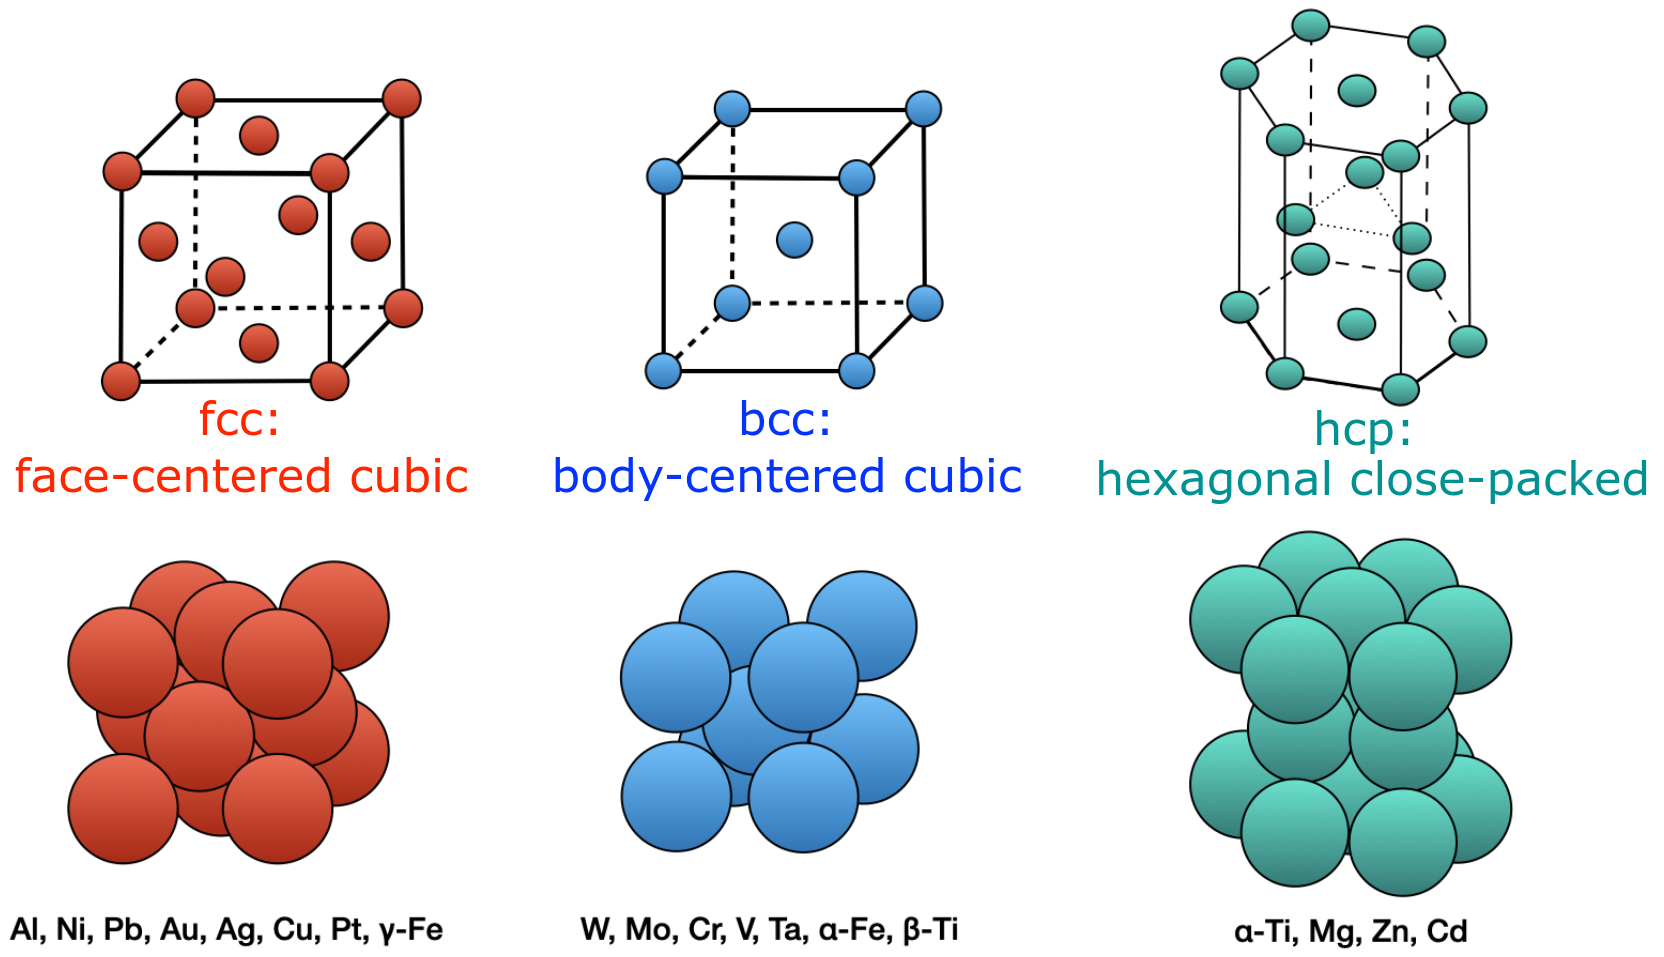
\includegraphics[width=0.71\textwidth]{media/fccbcchcp.png}
\end{center}

\begin{minipage}[t]{0.33\textwidth}
  \pph{FCC (Face-centered cubic)}
  \begin{itemize}
    \item Packing efficiency:\\[0.1cm]
      $\phi = \dfrac{\pi}{\sqrt{18}} \approx 74\%$
    \item Has many slip systems (12)
    \item Closest packed direction
  \end{itemize}
\end{minipage}%
\begin{minipage}[t]{0.33\textwidth}
  \pph{BCC (Body-centered cubic)}
  \begin{itemize}
    \item Packing efficiency:\\[0.1cm]
      $\phi = \dfrac{\sqrt{3\pi}}{8} \approx 68\%$
    \item Has many slip systems (6)
    \item Not closest packed direction
    \item Cottrell atmosphere
  \end{itemize}
\end{minipage}%
\begin{minipage}[t]{0.33\textwidth}
  \pph{HCP (Hexagonal close-packed)}
  \vspace*{-0.45cm}
  \begin{itemize}
    \item Packing efficiency:\\[0.1cm]
      $\phi = \dfrac{\pi}{\sqrt{18}} \approx 74\%$
    \item Very few slip systems (3)
    \item Closest packed direction
  \end{itemize}
\end{minipage}

\figbox{$\text{Packing efficiency}\, \left(\phi\right) = \dfrac{\text{Volume occupied by atoms in unit cell}}{\text{Total volume of unit cell}}$}
\newpage

\subsection{Structural model of ceramics}
In general, ceramics have:
\begin{itemize}
  \item \textbf{Ionic bonding, complex crystal structures (ceramics), amorphous (glasses)}
  \item Undoped: insulators (doped: semiconductors, superconductors or ionic conductors)
  \item Brittle, but high chemical and thermal resistance
  \item Wear-resistant, other special properties (e.g. ferro-/piezoelectricity)
\end{itemize}

\begin{figure*}[ht!]
  \centering
  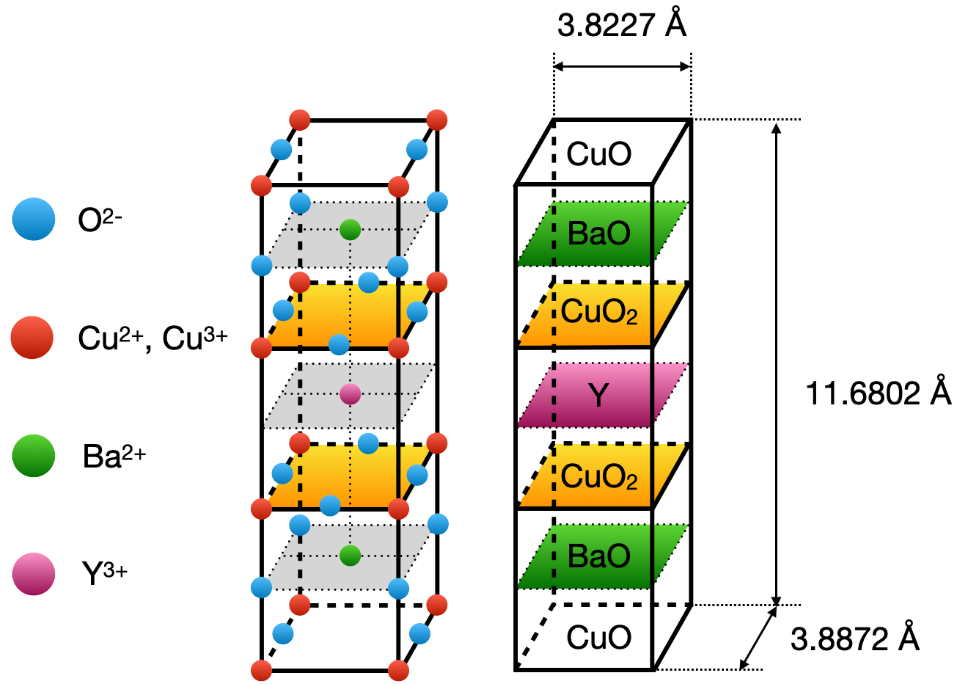
\includegraphics[width=0.6\textwidth]{media/ceramic_structure.png}
  \caption*{YBCO superconducting ceramic with layered perovskite-like structure}
\end{figure*}

\subsection{Structural model of polymers}
In general, polymers have:
\begin{itemize}
  \item Macromolecules ($10^3$ to $10^5$ C atoms)
  \item \textbf{Weaker intermolecular bonds} (strong atomic bond in molecular chain)
  \item Electrically and thermally insulating (without special modifications)
  \item Cheap, moldable, massive waste problem (e.g. ocean pollution)
  \item Matrix for many composite materials (recycling problem)
\end{itemize}
\begin{figure*}[ht!]
  \centering
  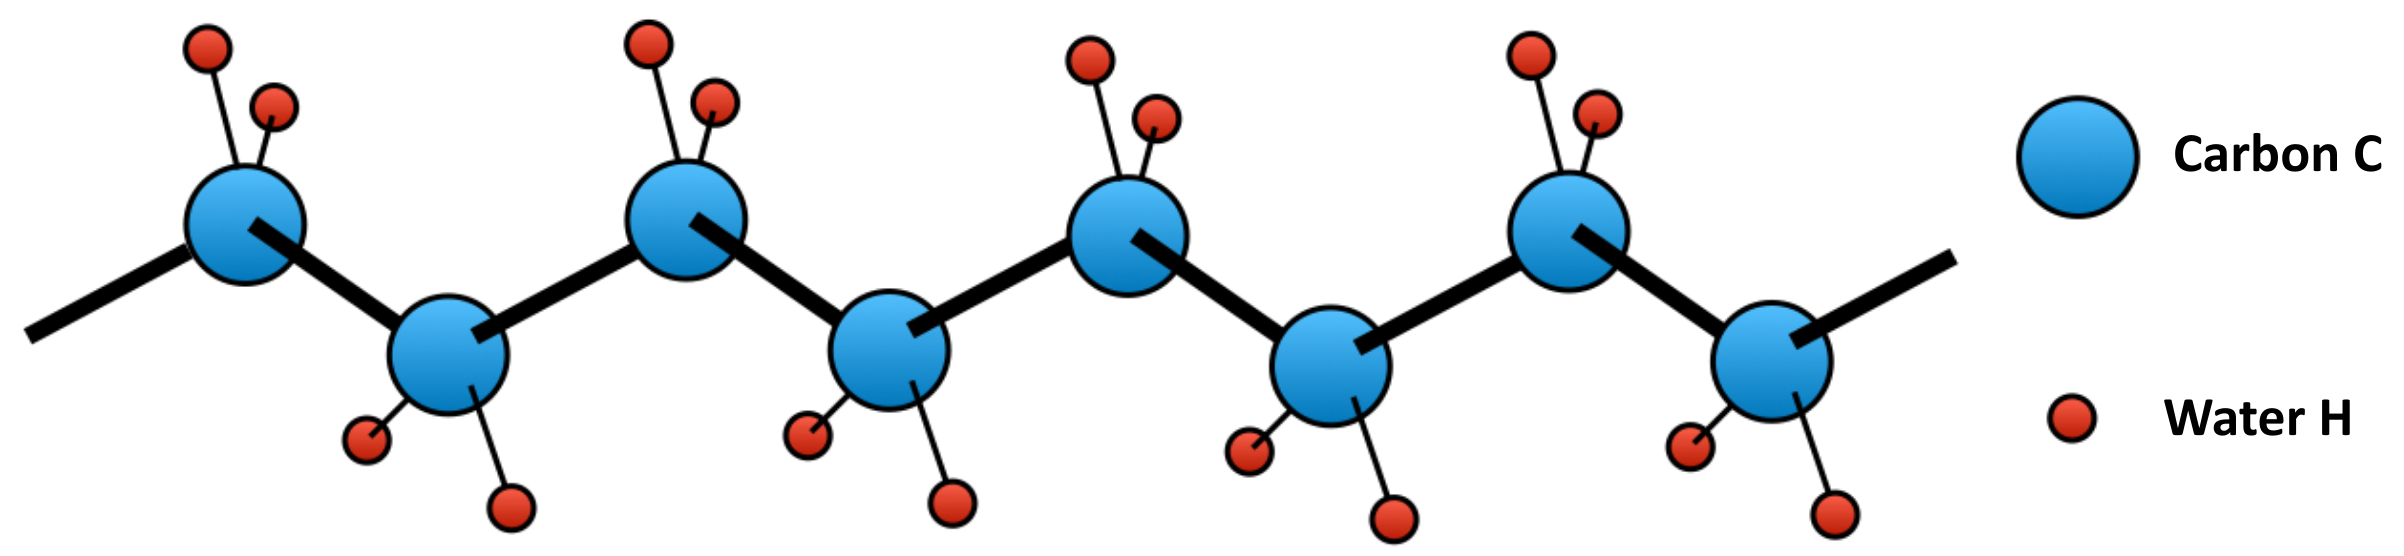
\includegraphics[width=0.8\textwidth]{media/polymer_structure.png}
  \caption*{Polymeric hydrocarbon chain}
\end{figure*}

\subsection{Amorphous and crystalline materials}
\begin{minipage}[t]{0.48\textwidth}
  \textbf{Amorphous materials}
  \begin{itemize}
    \item No crystal lattice (e.g. quartz glass, polymers)
    \item Atomic distances defined by chemical bonds
    \item Bond angles are variable
  \end{itemize}
\end{minipage}
\hfill
\begin{minipage}[t]{0.48\textwidth}
  \textbf{Crystalline materials}
  \begin{itemize}
    \item Crystal lattice (e.g. metals, ceramics, quartz)
    \item Atomic distances and bonding angles are defined
  \end{itemize}
\end{minipage}

\newpage
\begin{figure*}[ht!]
  \centering
  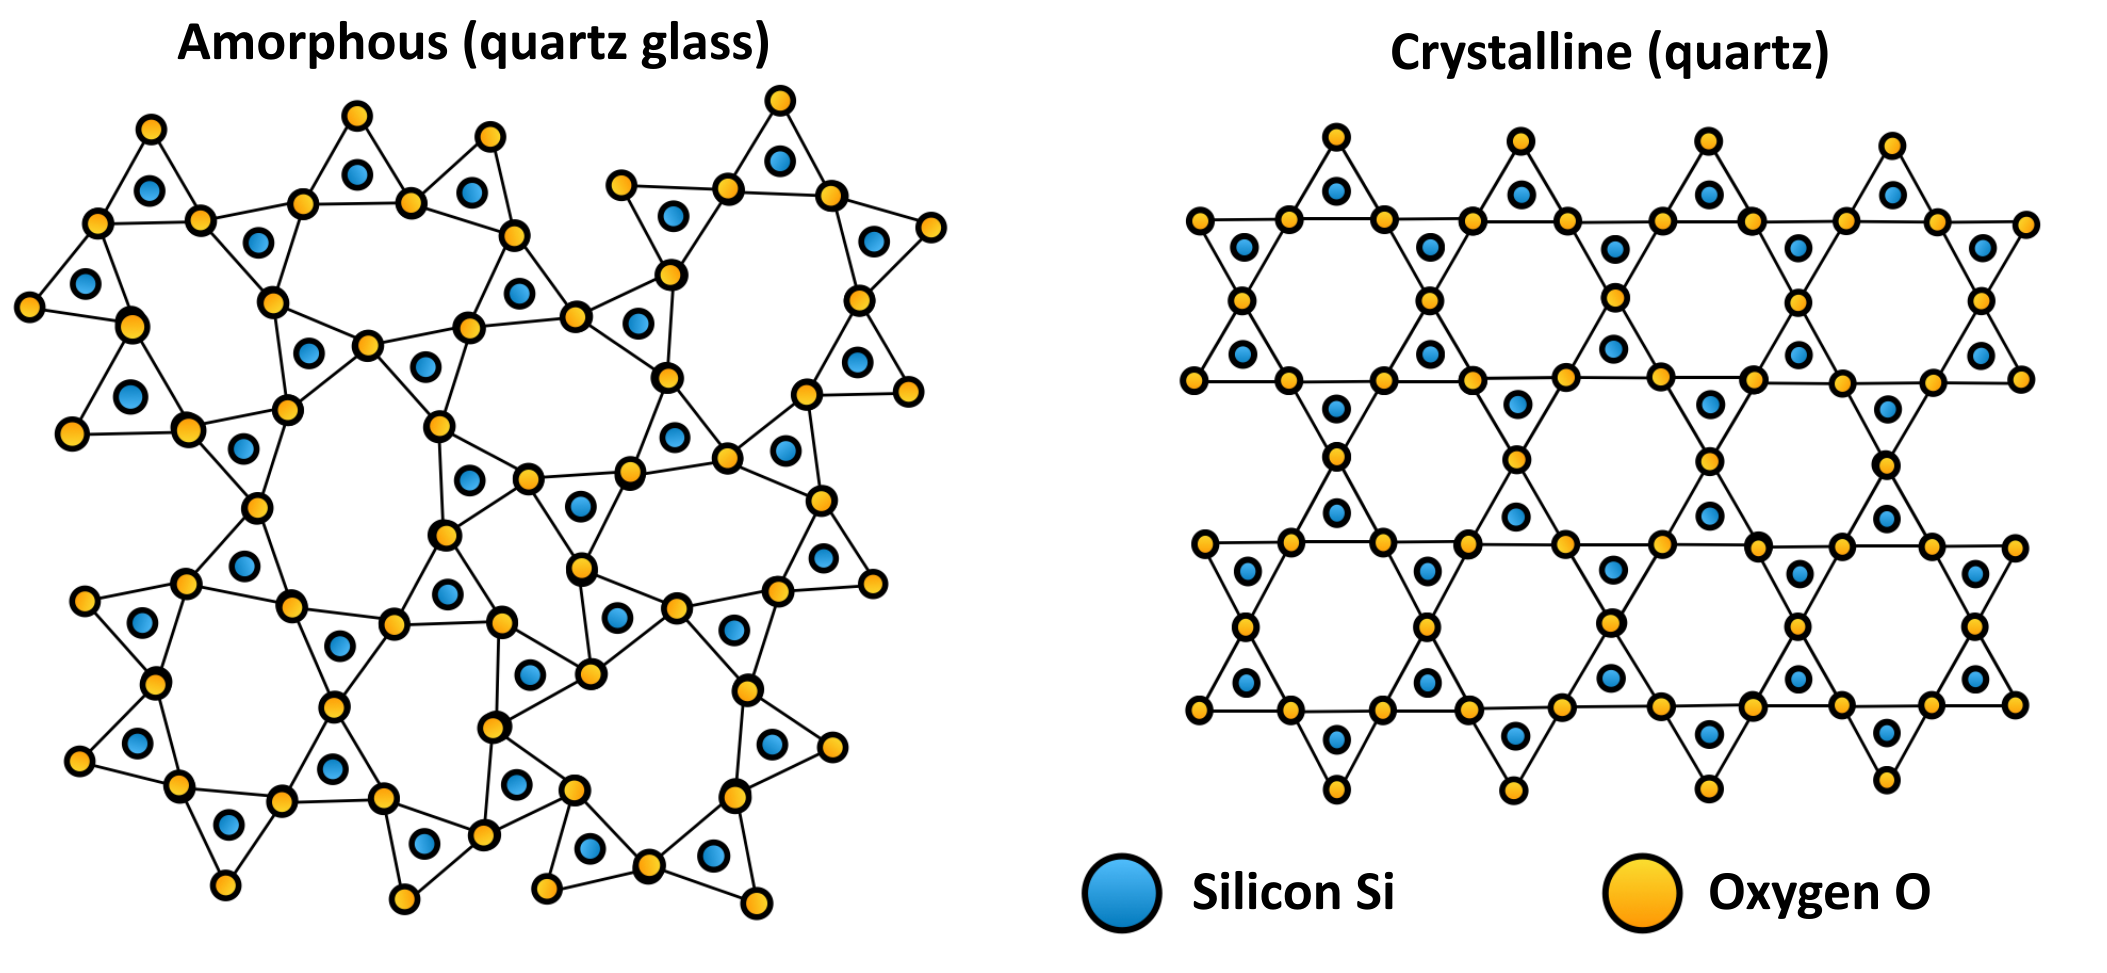
\includegraphics[width=0.8\textwidth]{media/amorph_cry.png}
\end{figure*}

\subsubsection{Polycrystalline materials}
Most metal components are polycrystalline (made of many grains/crystals),
i.e. they consist of countless microscopic crystals (crystallites, ``grains'').

\subsubsection{Monocrystalline materials}
\textbf{Only for special applications, expensive}
\begin{itemize}
  \item Single-crystal turbine blades ($T>1000^\circ C$, creep-resistant)
  \item Semiconductors, MEMS components made of silicon (e.g. gyroscopes in smartphones, accelerometers)
  \item Optical elements (e.g. laser crystals, $\lambda/4$ plates, crystals for frequency doubling of lasers)
\end{itemize}


\subsubsection{Amorphous materials}
\begin{itemize}
  \item Inorganic glasses (also Gorilla glass of smartphones)
  \item Metallic glasses (ferrous transformer sheet metal)
  \item Amorphous plastics (e.g. PMMA - plexiglass, COC, \dots)
\end{itemize}

\subsubsection{Structure difference}
\begin{figure*}[ht!]
  \centering
  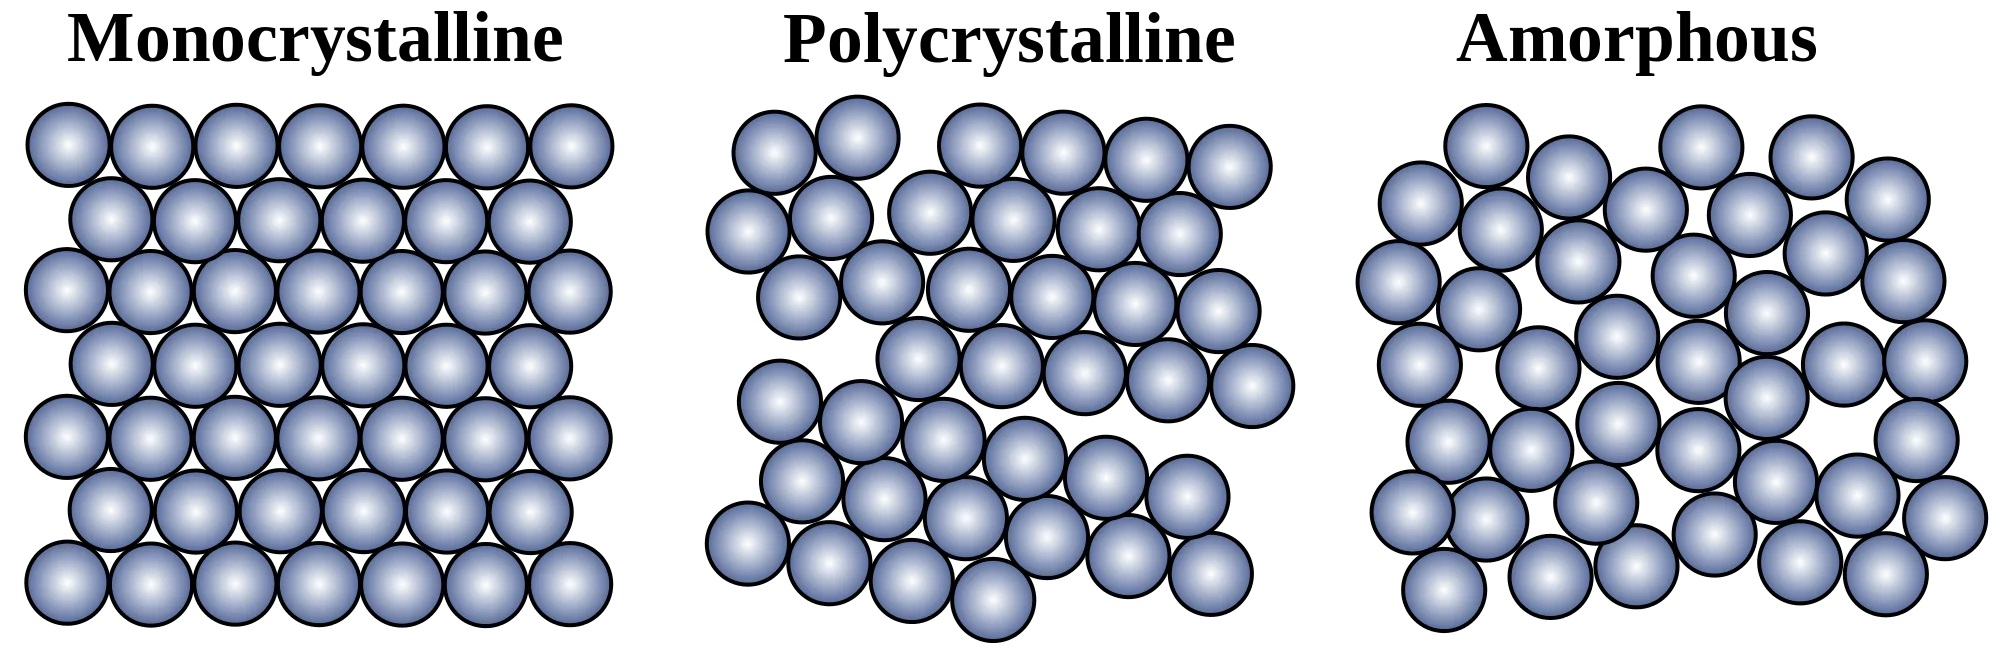
\includegraphics[width=0.8\textwidth]{media/mono_poly_amorph.jpg}
\end{figure*}

\subsection{Directionals dependence of the properties of materials}
\subsubsection{Anisotropy and Isotropy}
\begin{itemize}
  \item Anisotropic: Properties depend on direction (e.g. single crystals, wood, composites)
  \item Isotropic: Properties do not depend on direction (e.g. polycrystalline metals, amorphous materials)
\end{itemize}

\subsubsection{Anisotropy of the Young's Modulus $E$ in most cubic crystals}
In most cases, the $E$ is the largest in the direction of the closest packed atomic planes,
in direction of the space diagonal $\langle 111 \rangle$.

\newpage
\subsubsection{Miller indices for crystal directions}
In short, the Miller indices are the reciprocals of the fractional intercepts
that the plane makes with the crystallographic axes:
\begin{figure*}[ht!]
  \centering
  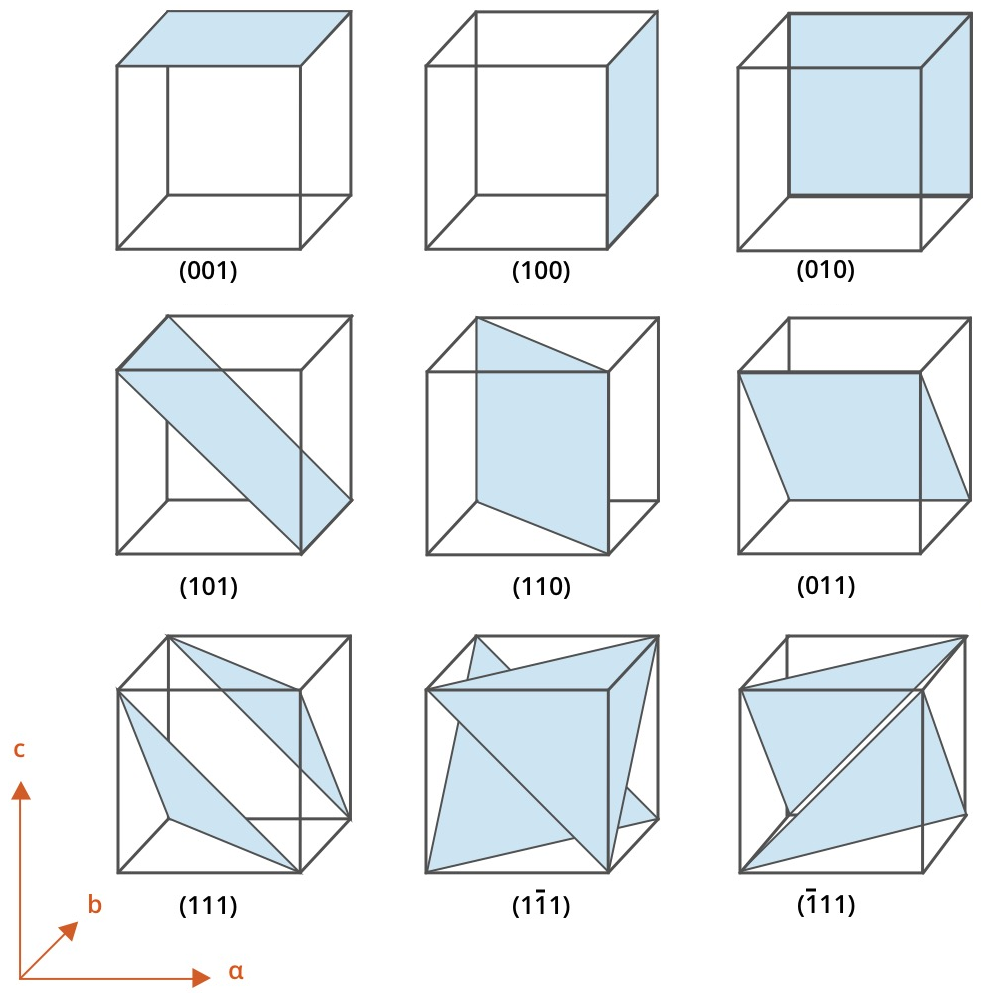
\includegraphics[width=0.5\textwidth]{media/miller_indices.png}
\end{figure*}

\subsection{Directional dependence of properties in polycrystalline materials}
\subsubsection{Polycrystalline materials without texture}
The polycrystalline materials without texture are considered \textbf{quasi-isotropic},
because the grains are randomly oriented.
\begin{figure*}[ht!]
  \centering
  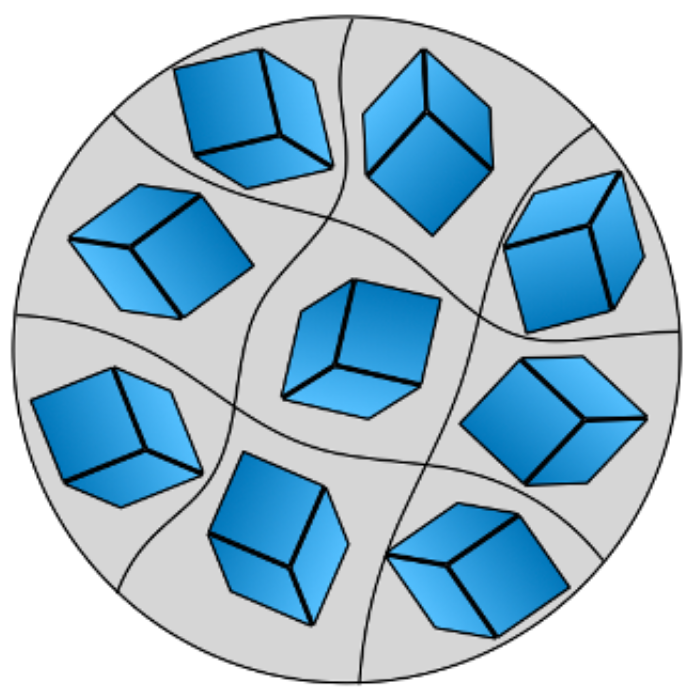
\includegraphics[width=0.1825\textwidth]{media/poly_notexture.png}
  \caption*{Polycrystalline material without texture}
\end{figure*}

\underline{Notice}: each crystal is anisotropic. but the material is quasi-isotropic to the outside, directional
dependence ``averages out''

\subsubsection{Polycrystalline materials with texture}
The polycrystalline materials with texture are considered \textbf{anisotropic},
because the grains are preferentially oriented.
\begin{figure*}[ht!]
  \centering
  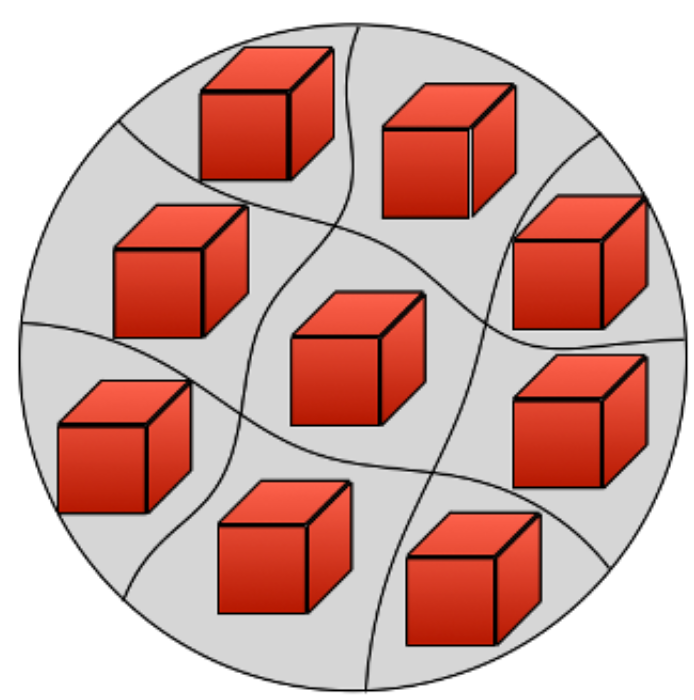
\includegraphics[width=0.1825\textwidth]{media/poly_texture.png}
  \caption*{Polycrystalline material with texture}
\end{figure*}
\newpage

\subsection{Material properties wrap-up}
\subsubsection{Single crystal materials}
\begin{itemize}
  \item \textbf{Anisotropic}
  \item Properties depend on direction
  \item Not uniform = anisotropic
\end{itemize}

\subsubsection{Polycrystalline materials without texture}
\begin{itemize}
  \item \textbf{Quasi-isotropic}
  \item Each crystal: anisotropic
  \item Uniform properties in all directions: isotropic \textrightarrow\ quasi-isotropic
\end{itemize}

\subsubsection{Polycrystalline materials with texture}
\begin{itemize}
  \item \textbf{Anisotropic}
  \item Preferential orientation of the crystallites: texture \textrightarrow\ anisotropic
  \item Examples: rolled and recrystallized electrical sheets with Goss texture
\end{itemize}

\subsubsection{Amorphous materials}
\begin{itemize}
  \item \textbf{Isotropic} (e.g. glass or amorphous metals)
\end{itemize}

\subsection{Polymorphism (Allotropy)}
Some materials may exhibit more than one crystal structure:
\begin{itemize}
  \item Iron $
    \begin{cases}
      \alpha\text{-Fe (ferrite, BCC)} & \text{below } 911^\circ\text{C} \\
      \gamma\text{-Fe (austenite, FCC)} & 911^\circ\text{C} \text{ to } 1392^\circ\text{C} \\
      \delta\text{-Fe (ferrite, BCC)} & 1392^\circ\text{C} \text{ to } 1536^\circ\text{C}
    \end{cases}$
  \item Titanium $
    \begin{cases}
      \text{HCP} & \text{below } 880^\circ\text{C} \\
      \text{BCC} & \text{above } 880^\circ\text{C}
    \end{cases}$
  \item Shape memory alloys (e.g. NiTi)
  \item Carbon (graphite, diamond, graphene, fullerene, CNT, \dots)
  \item Zirconia (high crack resistance due to phase transformation toughening)
  \item Ferro- and piezoelectric materials (e.g. PZT, quartz, \dots)
\end{itemize}

\subsubsection{Polymorphism of Iron (Fe)}
\begin{figure}[ht!]
\centering
\begin{minipage}[t]{0.48\textwidth}
  \centering
  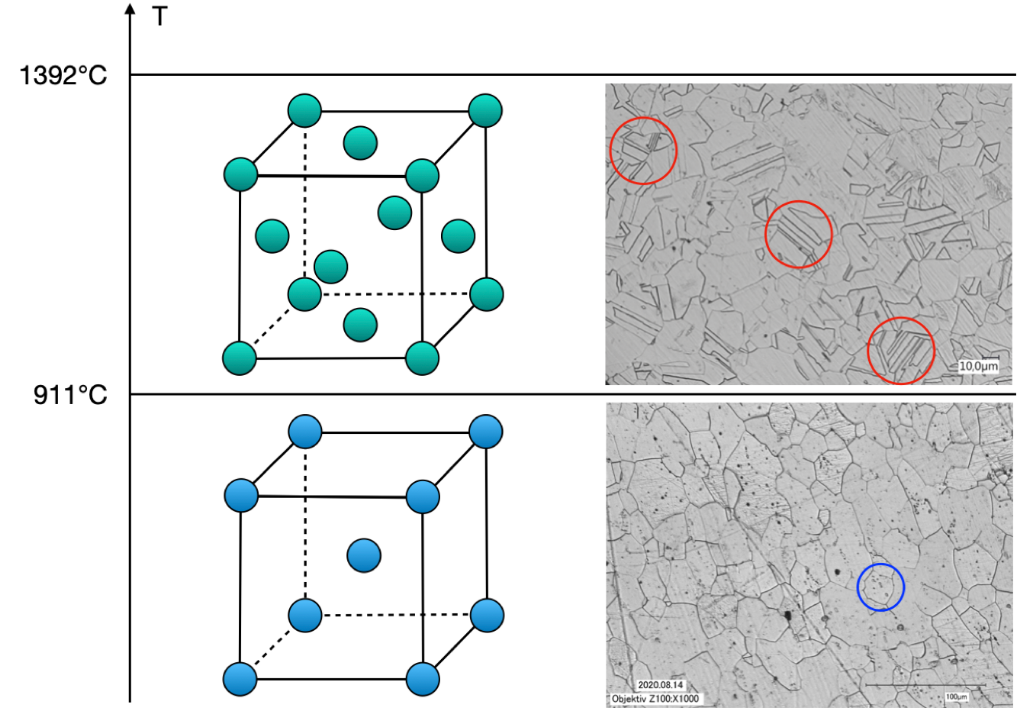
\includegraphics[width=\linewidth]{media/ferrite_trans.png}
  \captionof*{figure}{Slow Austenite transformation in steel: Ferrite}
\end{minipage}\hfill
\begin{minipage}[t]{0.48\textwidth}
  \centering
  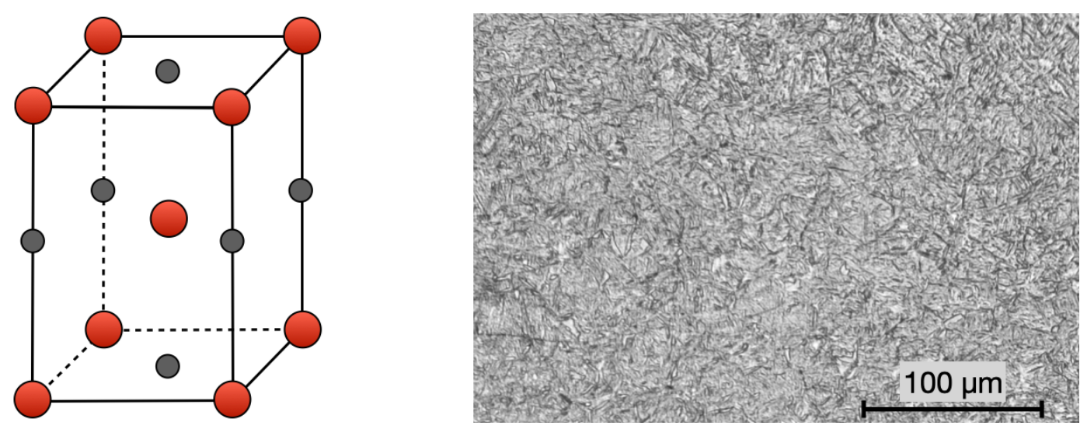
\includegraphics[width=\linewidth]{media/martenesite_trans.png}
  \captionof*{figure}{Fast Austenite transformation: Martensite}
\end{minipage}
\end{figure}

\newpage
\subsubsection{Polymorphism of Carbon (C)}
\forestset{
  mybox/.style={
    draw, rounded corners, align=center, inner sep=4pt, outer sep=2pt
  },
  my edge/.style={-latex}
}

\begin{forest}
for tree={
  mybox,
  edge={-latex},
  l sep=10pt,
  s sep=8pt,
  anchor=north
}
[Carbon
  [Amorphous Carbon
    [Activated Carbon]
    [Templated Carbon]
  ]
  [Crystalline Carbon
    [Graphite
      [Paracrystalline]
      [Rhombic]
      [Hexagonal]
    ]
    [Fullerene]
    [CNT]
    [Carbyne]
    [Diamond
      [Cubic]
      [Hexagonal]
    ]
  ]
]
\end{forest}

\subsubsection{Polymorphism of Nitinol (NiTi)}
NiTi is a shape memory alloy (SMA), used for screen lock of tablet notebooks, medtech,
and spectacle frames.
\begin{figure*}[ht!]
  \centering
  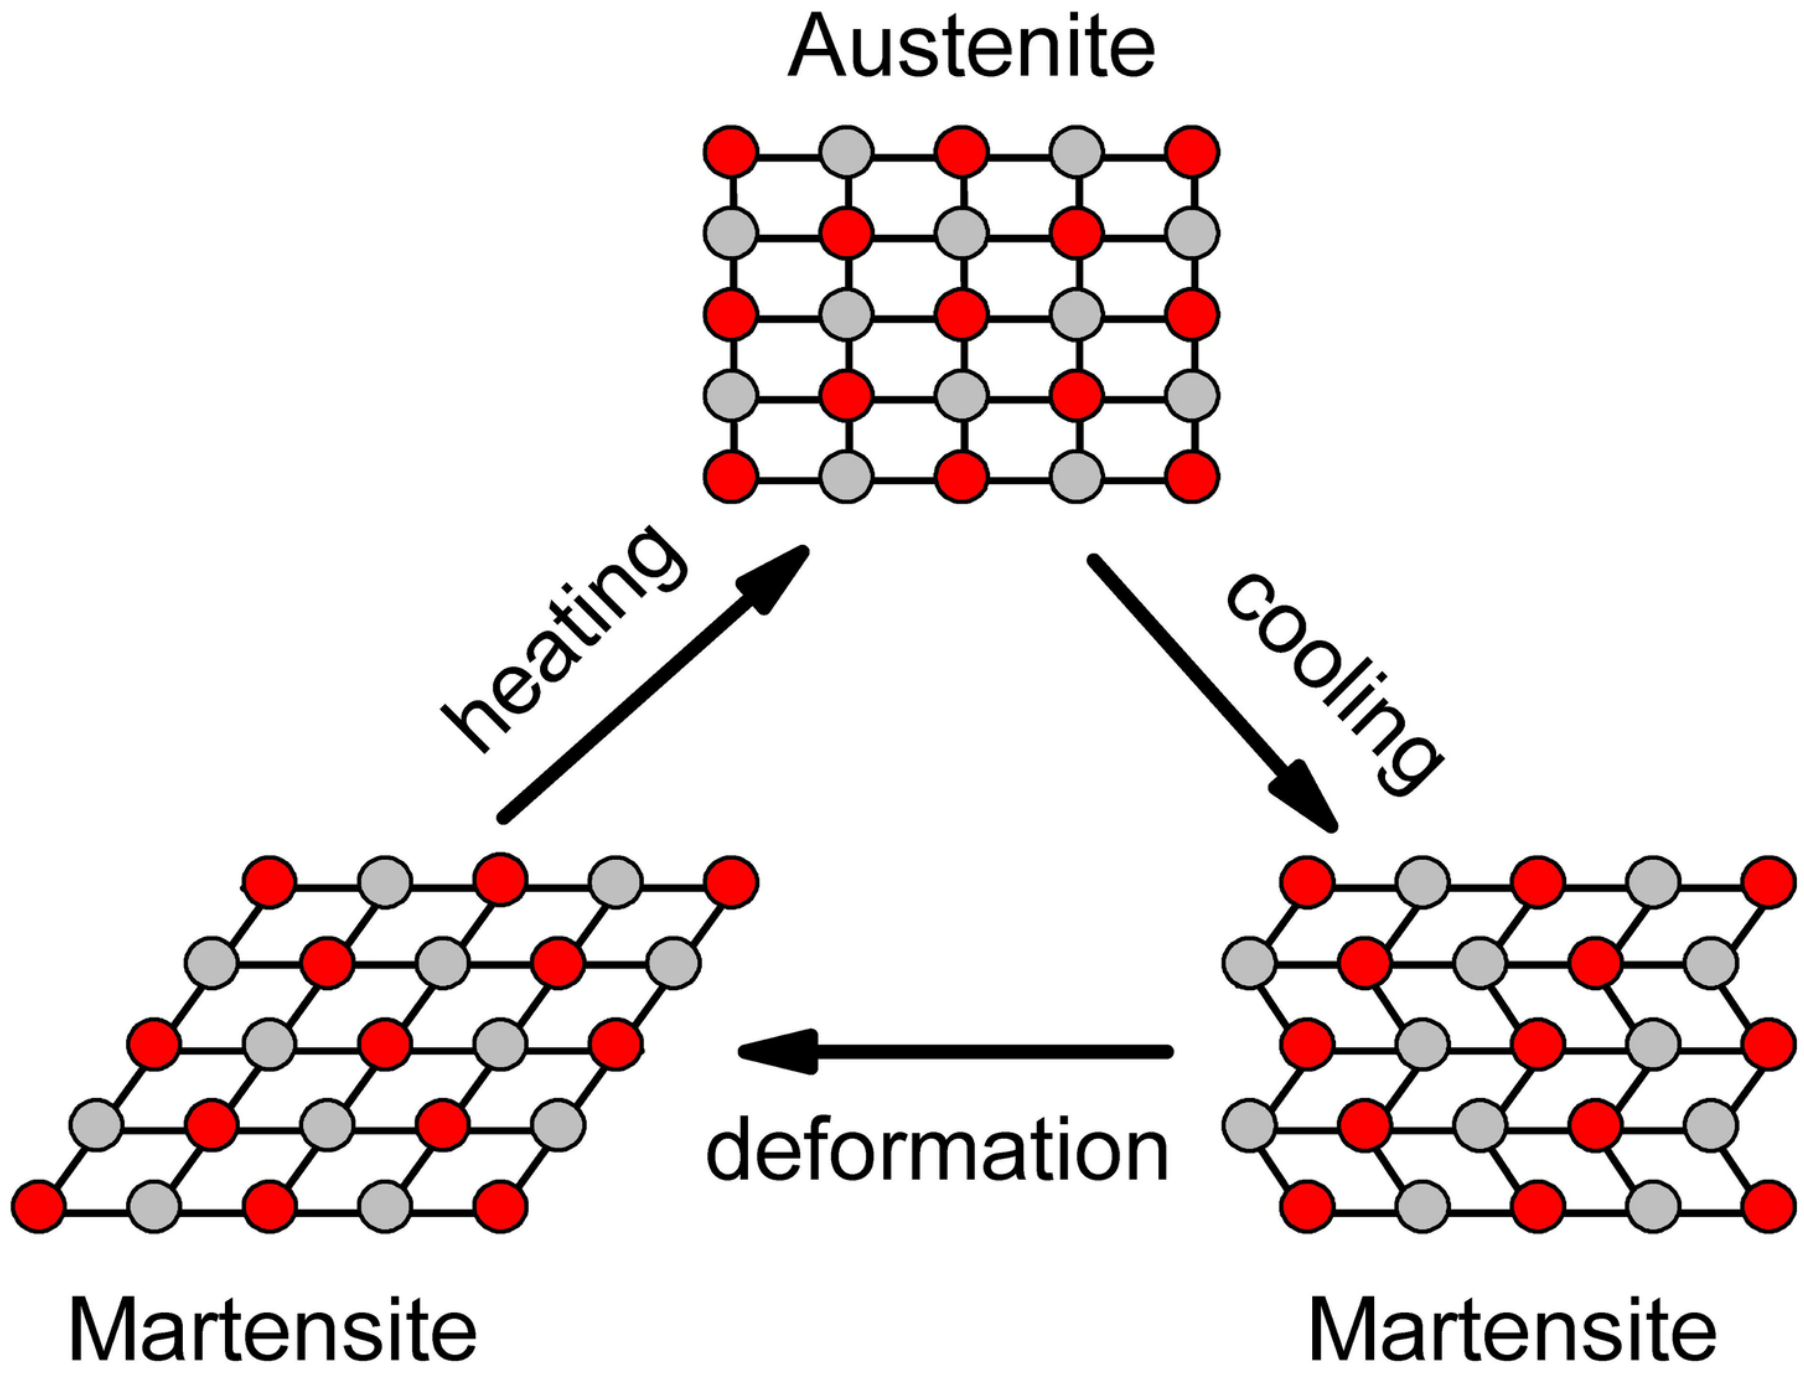
\includegraphics[width=0.4\textwidth]{media/Nitinol.png}
\end{figure*}

\subsection{Microstructure and Phases}
Phases are \textbf{homogeneous} subsections of a material with uniform physical and chemical properties:
\begin{itemize}
  \item A phase can be crystalline or amorphous
  \item At the phase boundaries, a sudden change in structure, properties and chemical composition occurs
\end{itemize}

Polycristalline materials can consist of:
\begin{itemize}
  \item One phase (homogeneous microstructure, e.g. only iron crystals)
  \item Different phases (heterogeneous microstructure, e.g. graphite and iron)
\end{itemize}

\begin{minipage}[t]{0.48\textwidth}
  \subsubsection{Homogeneous microstructure}
  They have only one phase and crystal structure:
  \vspace*{0.8cm}
  \begin{center}
    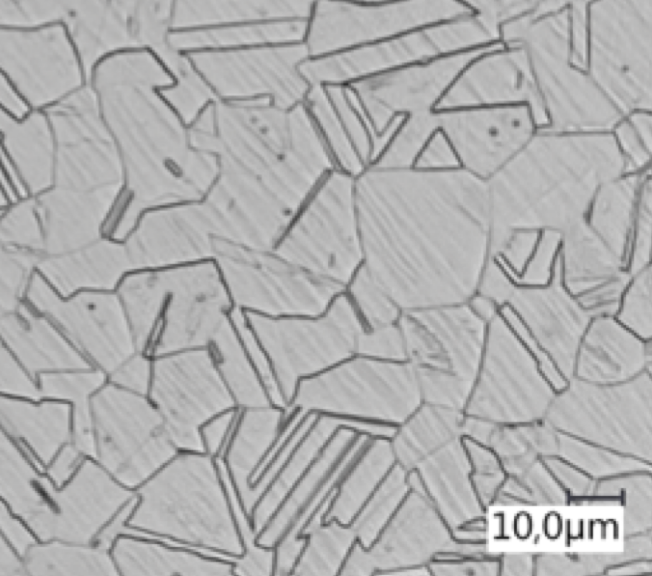
\includegraphics[width=0.65\textwidth]{media/homogeneous_microstructure.png}
  \end{center}
\end{minipage}
\hfill
\begin{minipage}[t]{0.48\textwidth}
  \subsubsection{Heterogeneous microstructure}
  They have multiple phases and many types of crystal structures:
  \vspace*{0.5cm}
  \begin{center}
    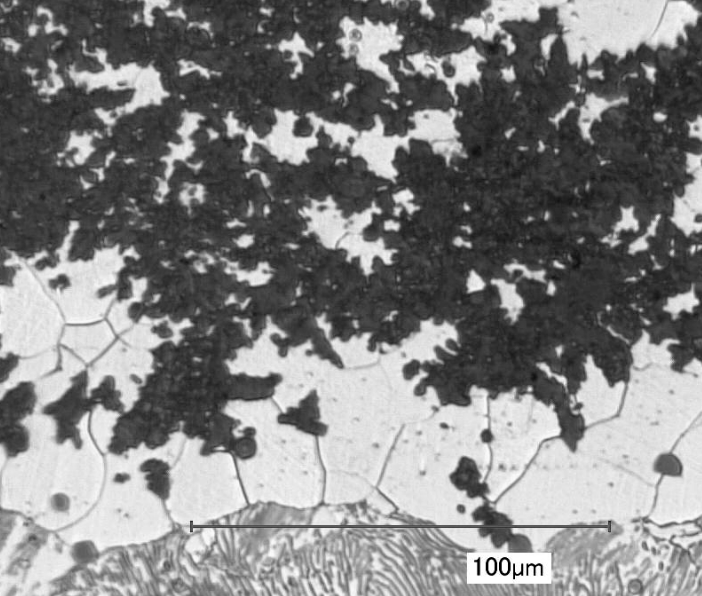
\includegraphics[width=0.7\textwidth]{media/heterogeneous_microstructure.png}
  \end{center}
\end{minipage}

\newpage
\subsection{Alloys}
\subsubsection{Definition of an alloy}
An alloy is a metallic material of at least 2 types of atoms:
\begin{itemize}
  \item Metal + Metal (iron-nickel, gold-silver, tin-lead, aluminum-copper, \dots)
  \item Metal + Non-metal (iron-carbon (steel), nickel-phosphorus, \dots)
\end{itemize}

\subsubsection{Microstructure of alloys}
\begin{itemize}
  \item \textbf{Homogeneous}, single-phase, only one type of cristal: SOLID SOLUTION CRYSTAL
  \item \textbf{Heterogeneous}, multi-phase, MIX OF DIFFERENT CRYSTAL TYPES:
  \begin{itemize}
    \item Crystals of pure metals without impurity atoms (no solid solution crystals)
    \item Solid solution crystals with impurity atoms,
    \item Crystals of intermetallic or intermediate phases (chem compounds crystals with their own distinguished crystal structure e.g. Ni$_3$Ti, Fe$_3$C, \dots)
    \item (Impurity particles, e.g. added ceramic particles or slag residues)
  \end{itemize}
\end{itemize}

\section{Most important metal structures and crystal lattice defects}
\subsection{Lattice defects}
Lattice defects are irregularities in the crystal structure:
\begin{itemize}
  \item \textbf{0-dimensional defects} (point defects)
  \item \textbf{1-dimensional defects} (line defects)
  \item \textbf{2-dimensional defects} (surface defects)
  \item \textbf{3-dimensional defects} (volume defects)
\end{itemize}

\subsubsection{0-dimensional defect}
0-dimensional defects include vacancies (missing atoms) and impurity atoms (foreign atoms in the lattice).

The approximate atomic size is 0.1nm.

\begin{figure*}[ht!]
  \centering
  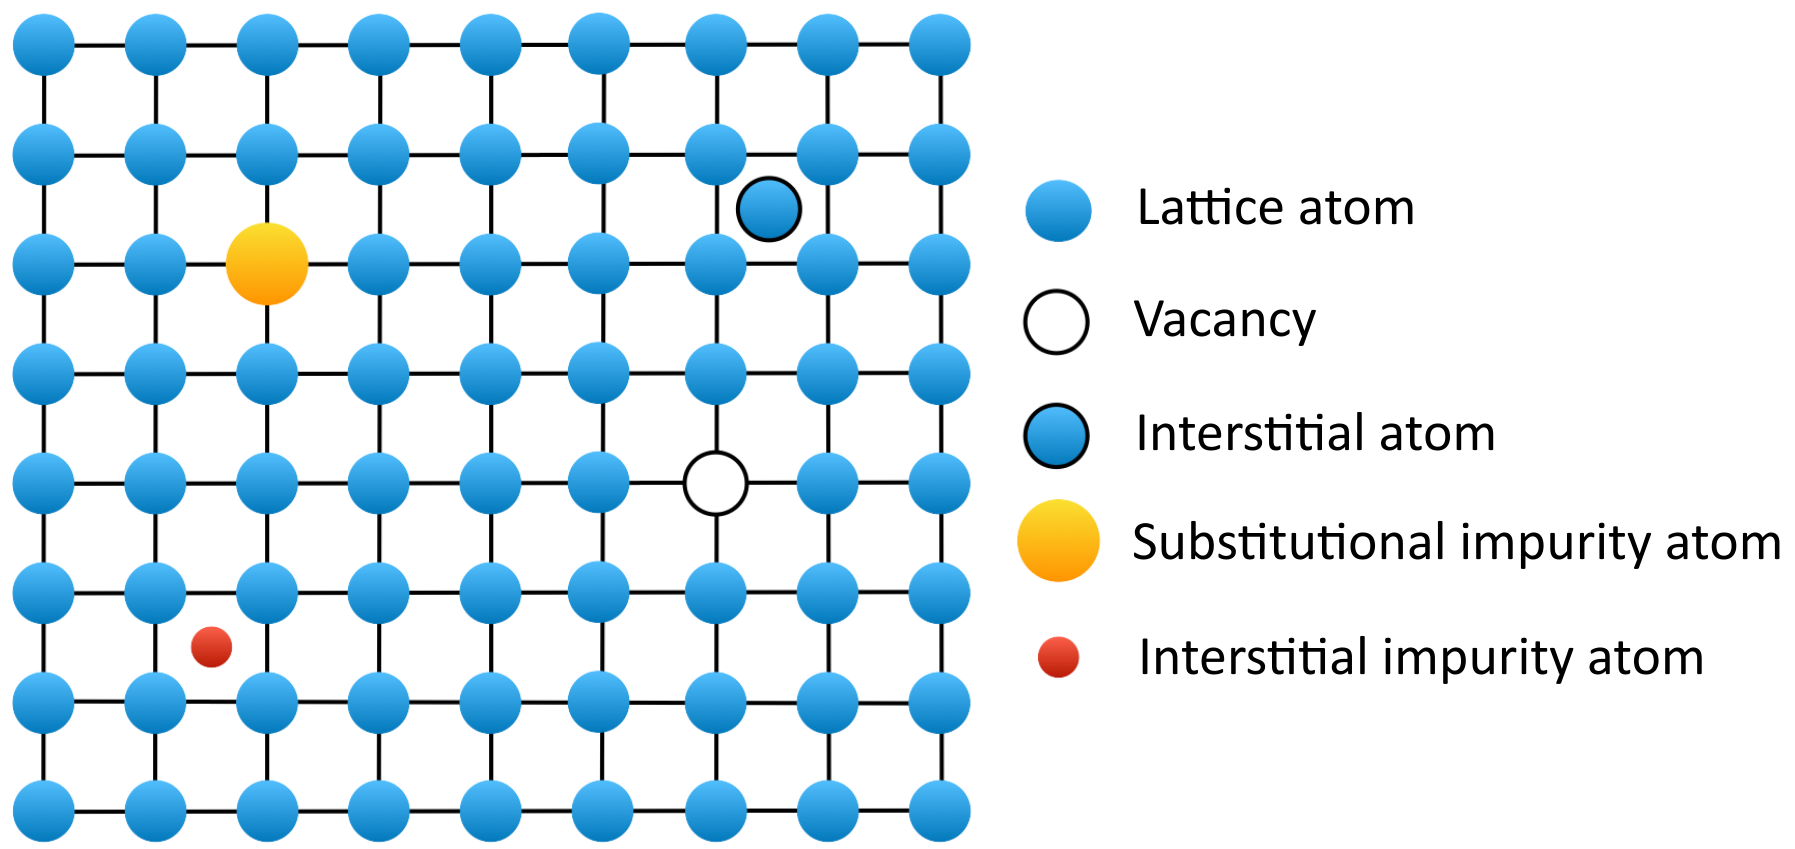
\includegraphics[width=0.6\textwidth]{media/lattice_0d.png}
  \caption*{Point defects: vacancy, interstitial atom, substitutional atom}
\end{figure*}

\newpage
\subsubsection{1-dimensional defect}
1-dimensional defects are dislocations (line defects) in the crystal structure.

Edge dislocations insert an extra half-plane of atoms in the crystal,
distorting the nearby planes of atoms.

\begin{figure*}[ht!]
  \centering
  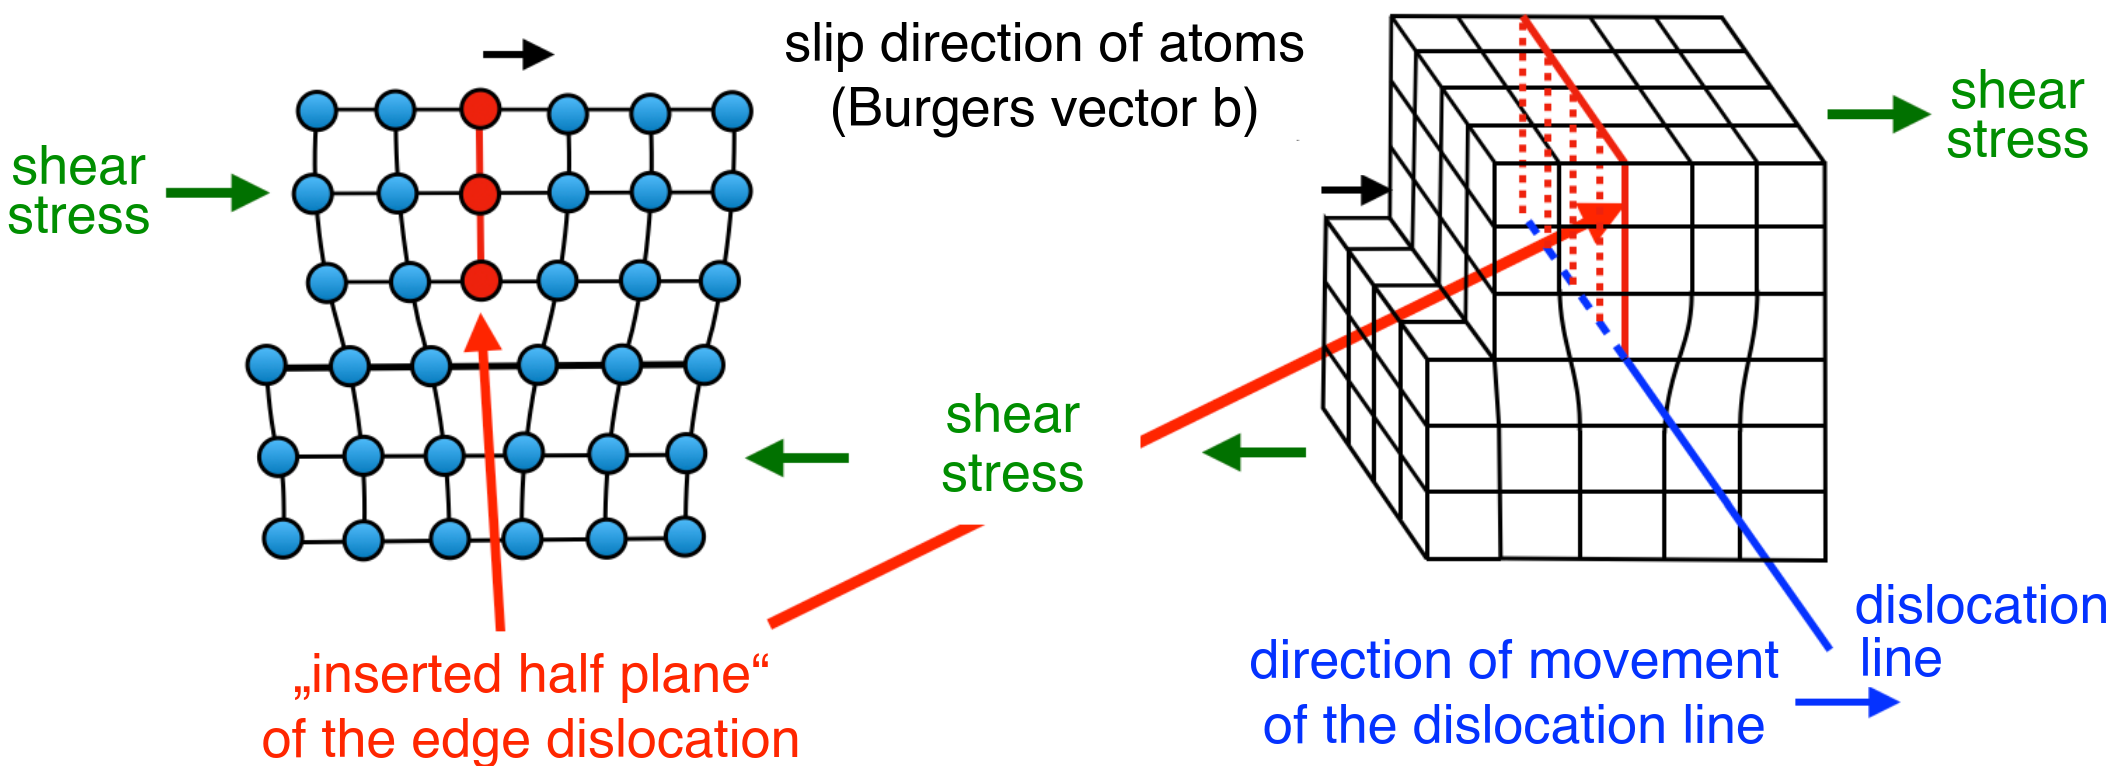
\includegraphics[width=0.8\textwidth]{media/lattice_1d.png}
  \caption*{Line defects: edge dislocation, screw dislocation}
\end{figure*}

\subsubsection{2-dimensional defect}
2-dimensional defects are grain boundaries (surface defects) in polycrystalline materials:
\begin{itemize}
  \item Crystal growth starts at multiple locations within the molten metal.
  \item Finally, the growing grains merge to form the microstructure of the solid metal.
\end{itemize}

The approximate atomic size is 10 to 100 $\mu$m.

\begin{figure*}[ht!]
  \centering
  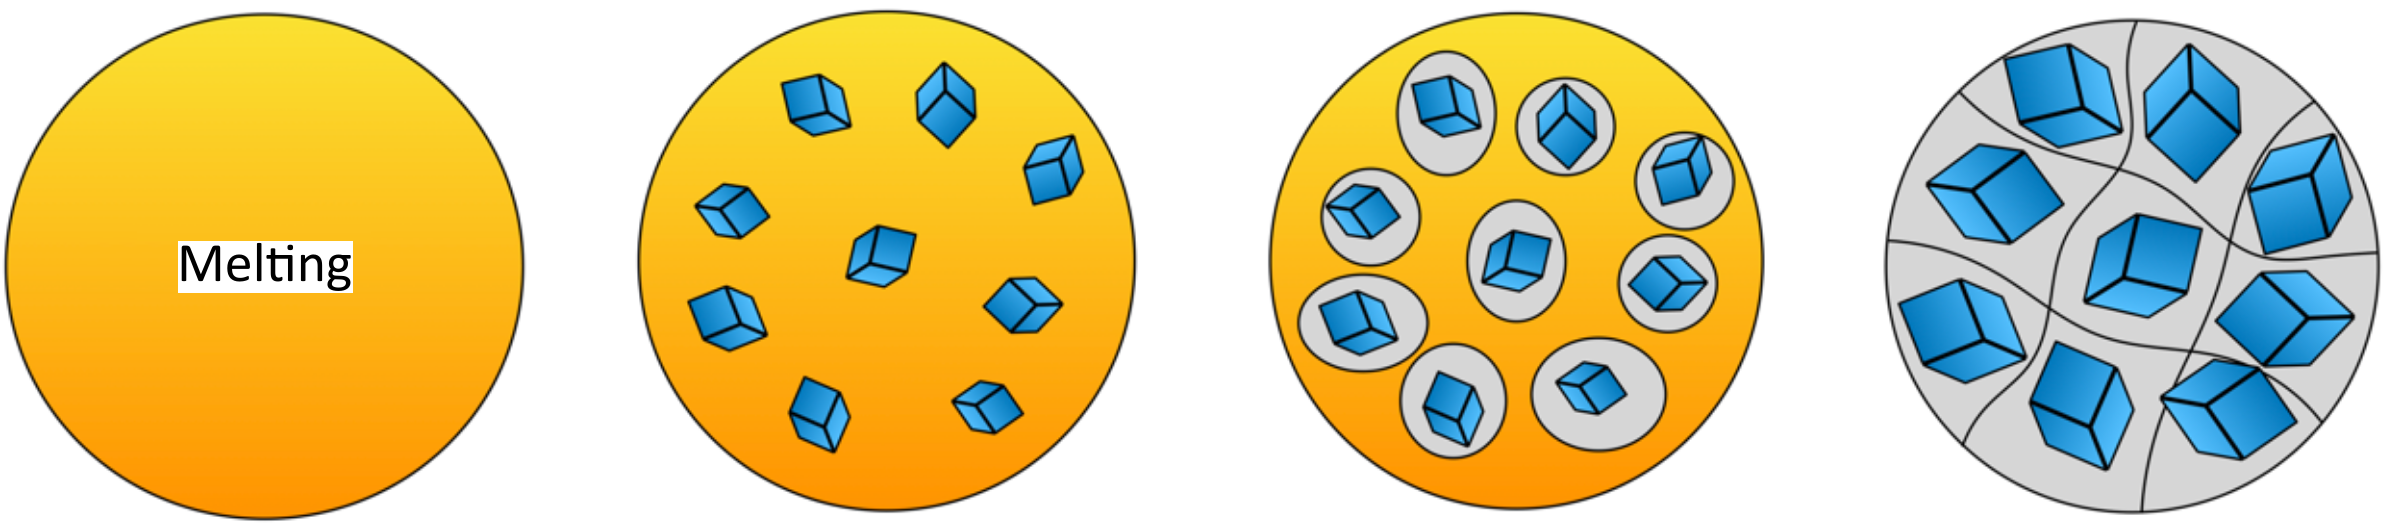
\includegraphics[width=0.8\textwidth]{media/lattice_2d.png}
  \caption*{Crystallization from a melt:\\(1) homogeneous melt, (2) nucleation of crystals, (3) crystal growth surrounded by residual melt, (4) fully solidified polycrystalline structure with grain boundaries}
\end{figure*}

\subsubsection{3-dimensional defect}
3-dimensional defects are precipitates, inclusions, voids, cracks (volume defects) in the crystal structure.

The size is very small (nanometers)
\begin{figure*}[ht!]
  \centering
  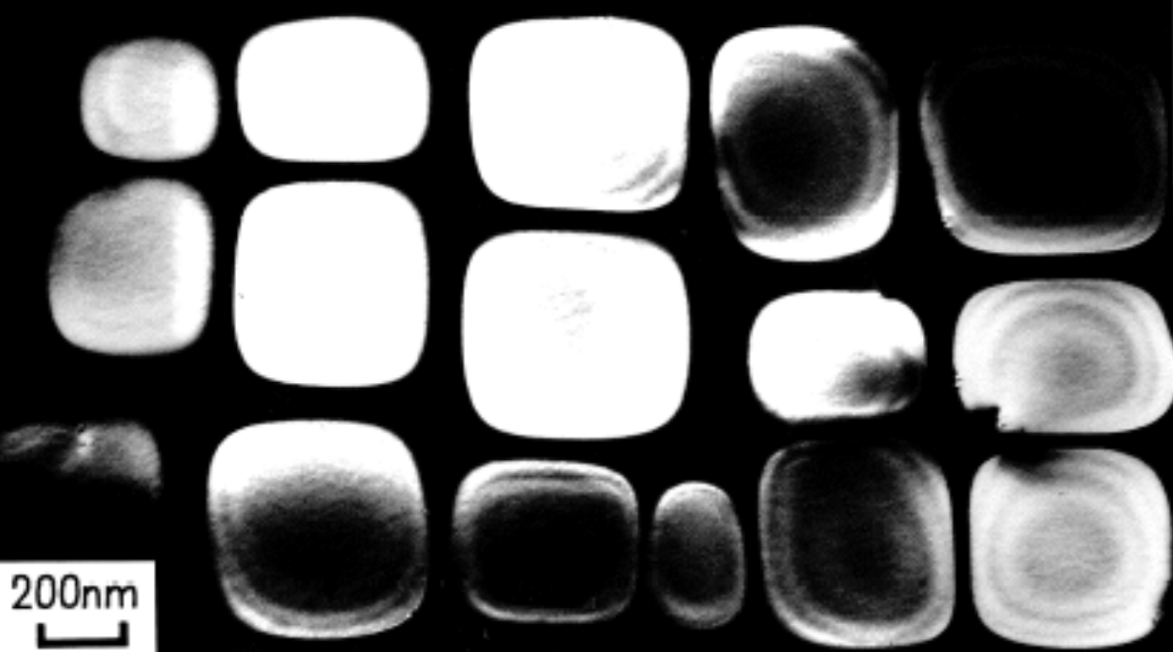
\includegraphics[width=0.55\textwidth]{media/lattice_3d.png}
  \caption*{Coherent Ni$_3$Al precipitates (white) in a Ni solid solution crystal (black)}
\end{figure*}

\newpage
\begin{wrapfigure}{l}{0.55\textwidth}
  \section{Elastic and plastic deformation}
  \subsection{Elastic deformation}
  \subsubsection{Atomic energy-distance model}
  The atomic energy-distance model describes the interaction between two atoms.

  The coefficient of thermal expansion $\alpha$ is inversely proportional to:
  \begin{itemize}
    \item Young's modulus $E$ (in case of springs, the force)
    \item Bonding energy
    \item Melting temperature
  \end{itemize}
\end{wrapfigure}

\phantom{}

\begin{figure*}[ht!]
  \begin{flushright}
    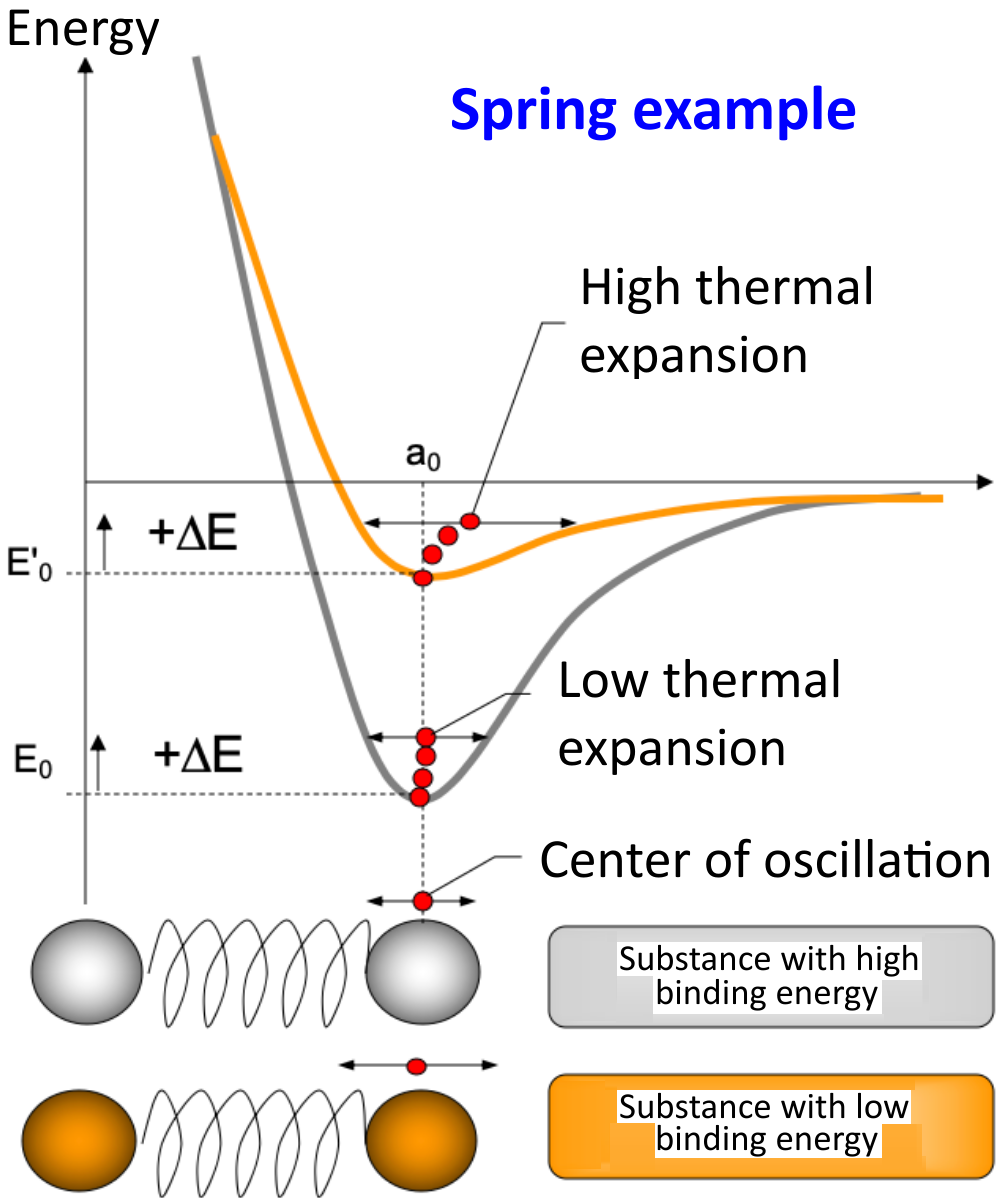
\includegraphics[width=0.4\textwidth]{media/atomic_energy_distance.png}
  \end{flushright}
\end{figure*}
\wrapfill

\vspace*{-8.6cm}

\subsection{Elastic constants of isotropic materials}
\subsubsection{Elastic stress, strain, and Young's modulus}
Letting the load be unidirectional and in x-direction, then:
\figbox{$\varepsilon_x = \dfrac{1}{E}\cdot \sigma_x\ \Longleftrightarrow\ \sigma_x = E \cdot \varepsilon_x$}

\subsubsection{Poisson's ratio $\nu$}
When a material is stretched in one direction (x-direction), it tends to contract in the other two directions (y- and z-directions).

The ratio of the transverse strain to the axial strain is called Poisson's ratio:
\figbox{$\nu = -\dfrac{\varepsilon_y}{\varepsilon_x} = -\dfrac{\varepsilon_z}{\varepsilon_x}$}

\subsubsection{Relationship between the 3 isotropic elastic constants $G$}
For isotropic materials, the following relationships hold:
\figbox{$G = \dfrac{E}{2(1+\nu)} = \dfrac{\sigma_x}{2\varepsilon_x(1+\nu)}$}

\subsection{Plastic deformation in metals}
The plastic deformation has as characteristics to be permanent and non-reversible.

\subsubsection{At room temperature}
\begin{itemize}
  \item Dislocations move on densely packed slip planes in densely packed directions
  \item Smaller slip distances require less external force or energy
\end{itemize}

\underline{Note}: There are exceptions. For example, metals with relatively low stacking
fault energy show:
\begin{itemize}
  \item Twin formation (e.g. nitinol)
  \item Partial dislocations pairs with stacking faults in between (e.g. Ni, Cu)
\end{itemize}

\subsubsection{At high temperatures}
The metal creeps, leading to diffusion of atoms, especially at grain boundaries.

\newpage
\subsection{Dislocation Slip Model}
The dislocation slip model describes the plastic deformation of metals by dislocation motion.

\subsubsection{Simplified model}
The simplified dislocation slip model is sufficient for practical understanding of plastic deformation:
\begin{itemize}
  \item Inserted half-plane, the end of which forms the dislocation line
  \item Dislocation moves on densely packed slip planes
\end{itemize}

\begin{figure*}[ht!]
  \centering
  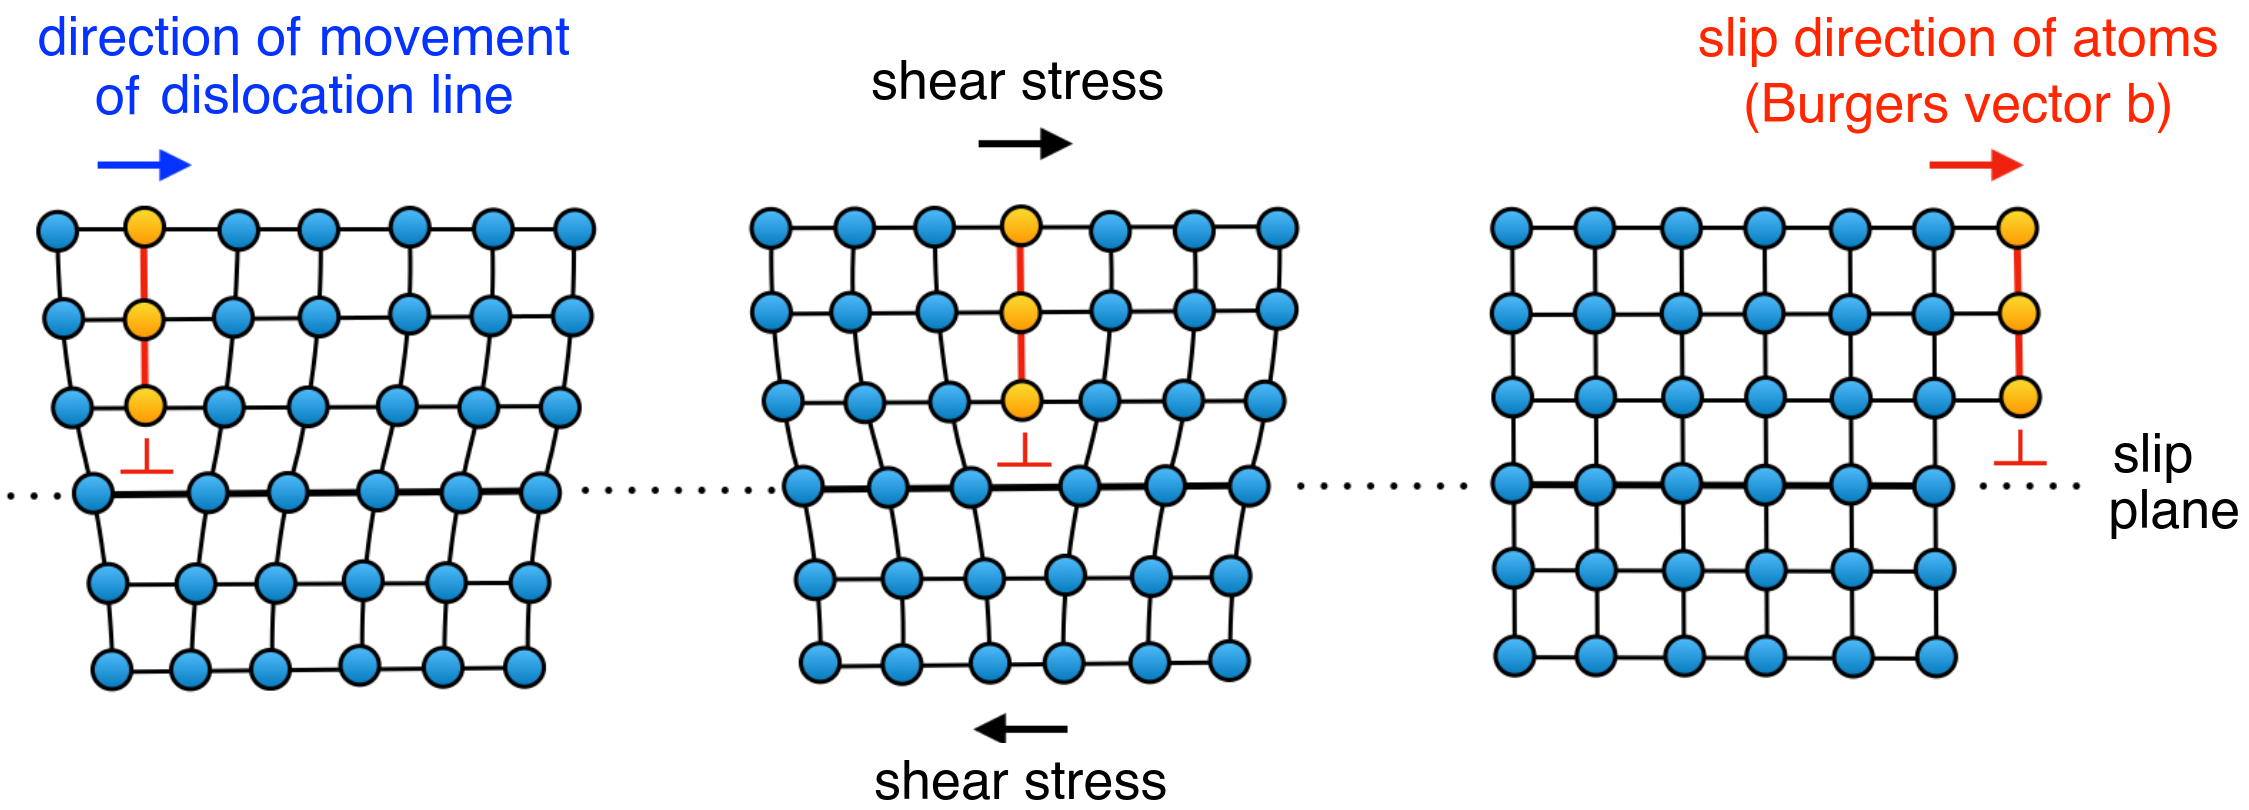
\includegraphics[width=0.8\textwidth]{media/simplified_dislocation_slip_model.png}
  \caption*{Edge dislocation motion under shear stress}
\end{figure*}

\subsection{Slip systems}
\subsubsection{Slip systems in FCC metals (Miller indices)}
FCC metals have 12 close-packed slip systems, making them soft and highly ductile (e.g. Au, Ag, Cu, Al, $\alpha$-Fe)
\begin{figure*}[ht!]
  \centering
  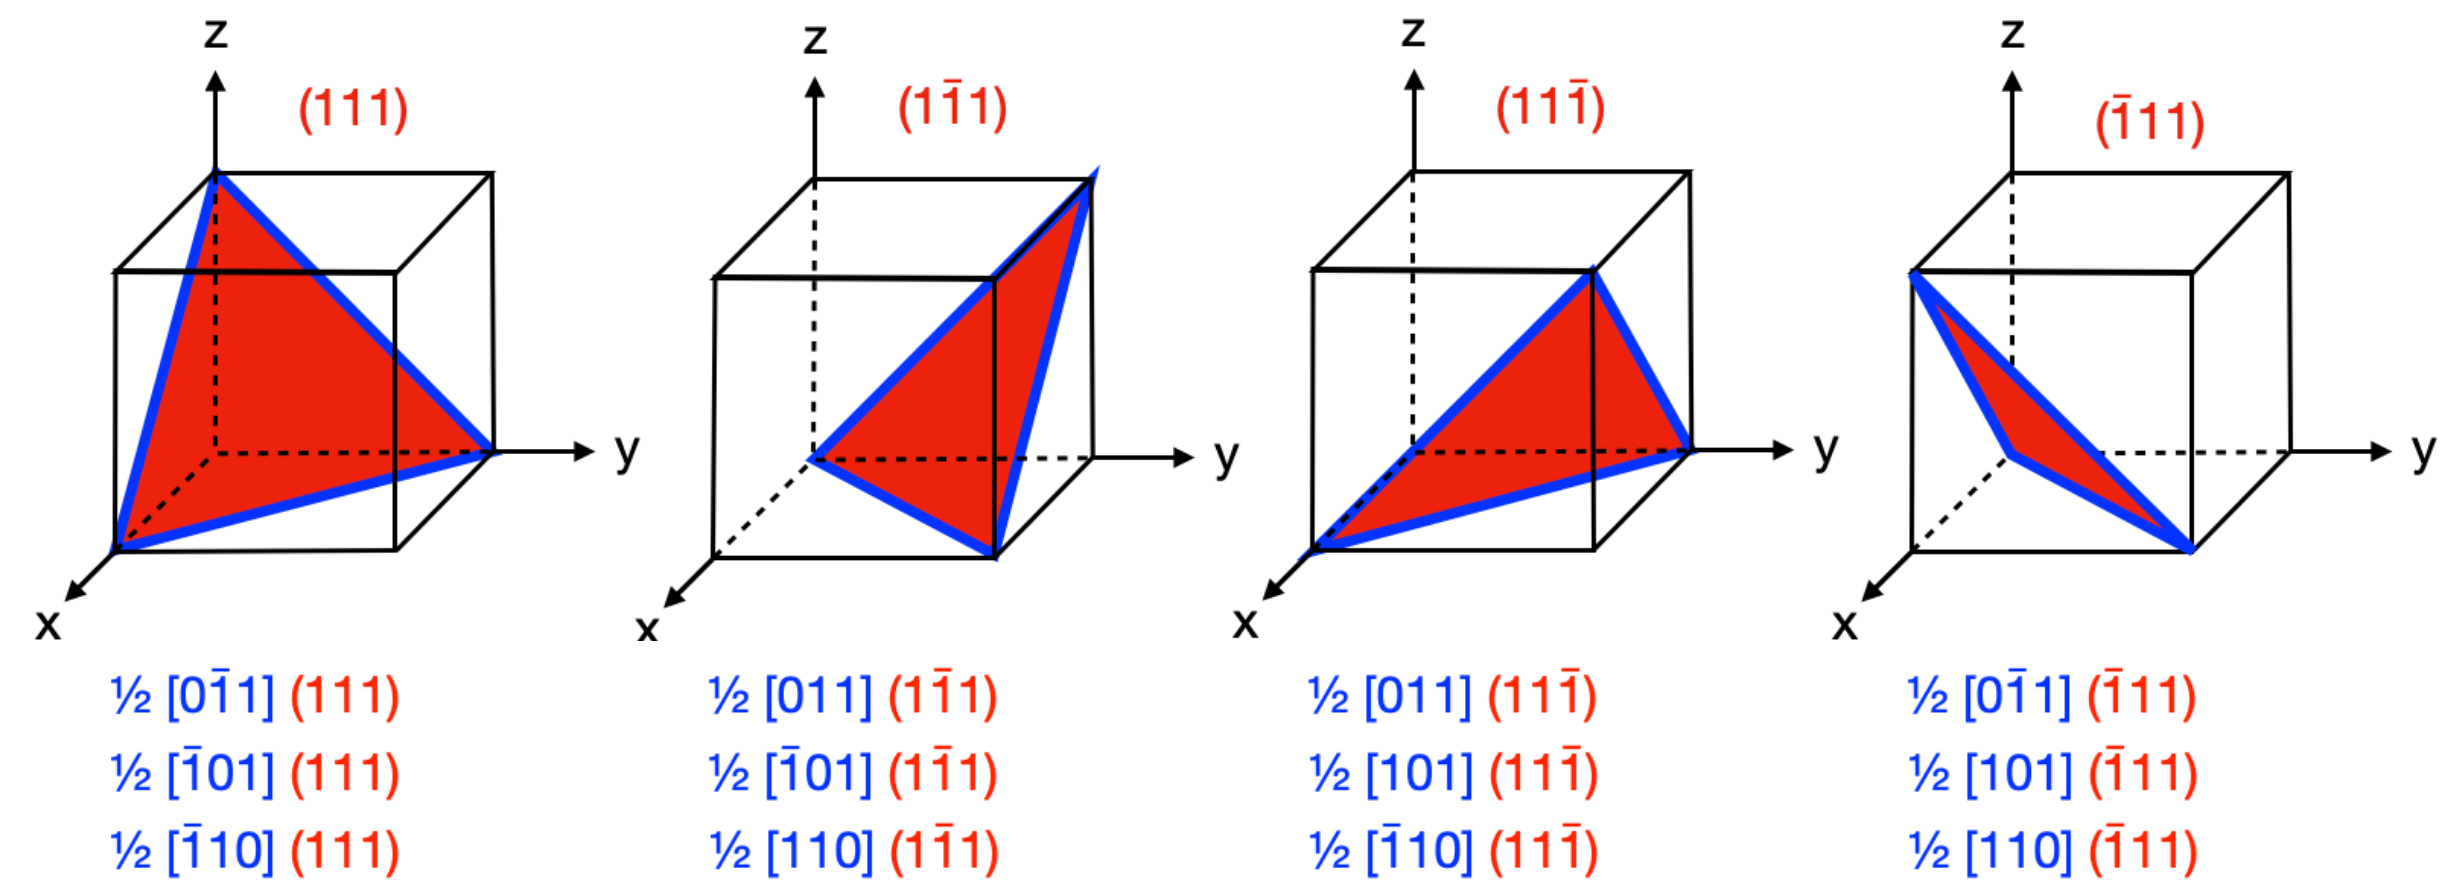
\includegraphics[width=0.8\textwidth]{media/FBB_miller.png}
\end{figure*}

\subsubsection{Slip systems in HCP metals (Miller indices)}
HCP metals are closely packed but deform on only one slip plane with 3 slip systems, resulting in limited ductility
(e.g. Ti, Zn, Mg). 
\begin{figure*}[ht!]
  \centering
  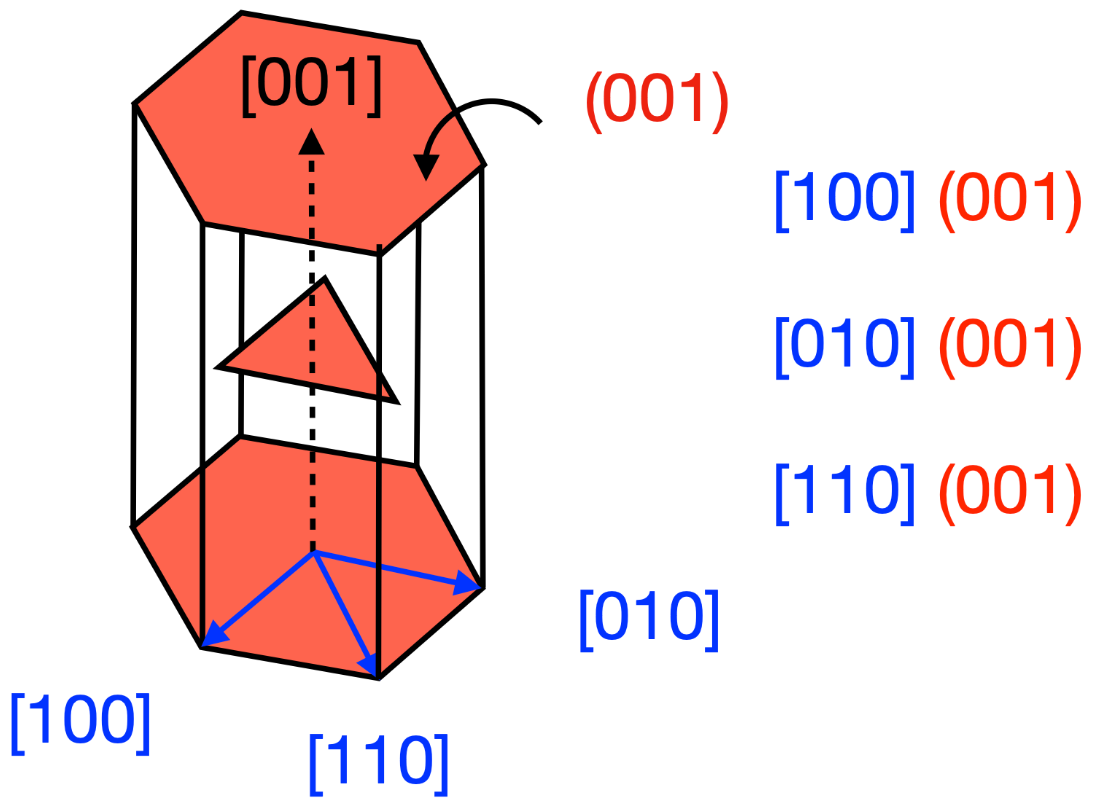
\includegraphics[width=0.35\textwidth]{media/HCP_miller.png}
\end{figure*}

\newpage
\subsubsection{Slip systems in BCC metals (Miller indices)}
BCC metals have 48 slip systems but are less closely packed, leading to higher strength
and lower ductility (e.g. $\alpha$-Fe, Cr, W, Mo, Ta, Nb)

\begin{minipage}[t]{0.6\textwidth}
  \centering
  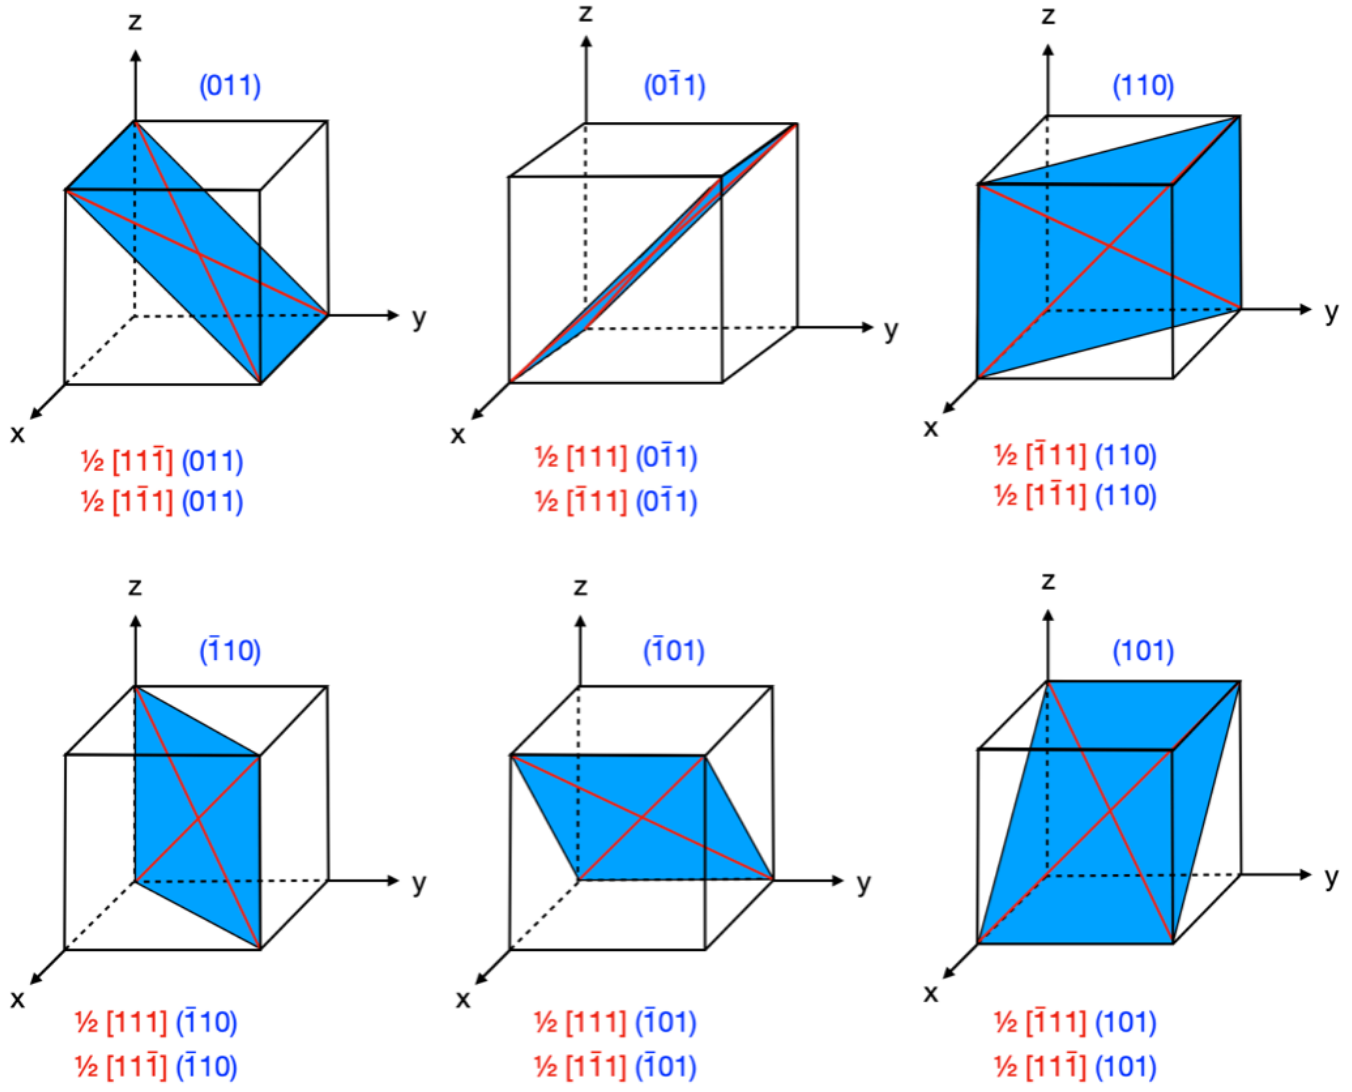
\includegraphics[width=\textwidth]{media/BCC_miller_major.png}
  \textbf{12 major slip systems:} 6 $\left\{110\right\}$ slip planes\\
  \textbf{2 slip directions:} $1/2 \langle 111 \rangle$ each
\end{minipage}
\begin{minipage}[t]{0.4\textwidth}
  \centering
  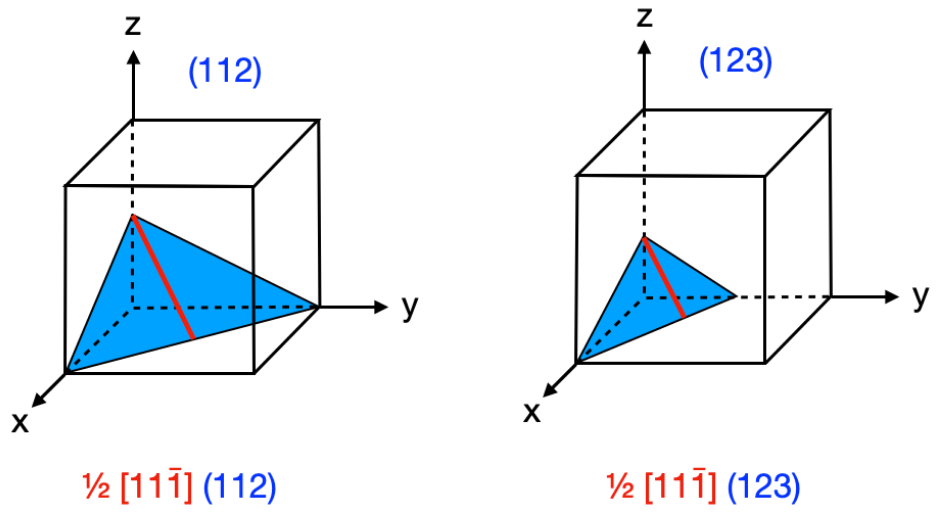
\includegraphics[width=\textwidth]{media/BCC_miller_minor.png}
  \textbf{36 minor slip systems:}\\
  12x $1/2 \langle111\rangle \left\{112\right\}$

  24x $1/2 \langle111\rangle \left\{123\right\}$
\end{minipage}

\begin{wrapfigure}{r}{0.2\textwidth}
  \centering
  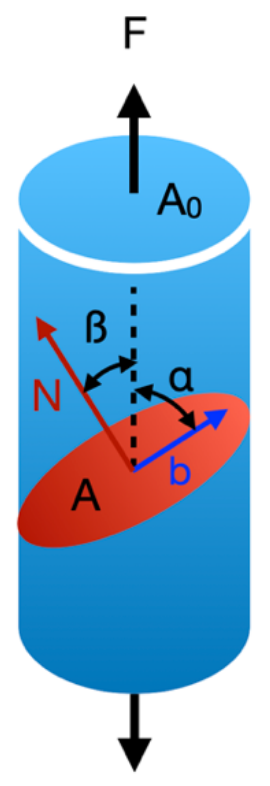
\includegraphics[width=0.5\linewidth]{media/schmids_law.png}
\end{wrapfigure}

\phantom{}

\subsection{Schmid's law of critical resolved shear stress}
The Schmid's law states that slip begins in a crystalline material when the resolved shear
stress on a slip system reaches a critical value.
\begin{itemize}
  \item PLastic deformation occurs only on closely packed slip planes where the applied
    shear stress exceeds a critical value
  \item Under uniaxial loading, the maximum shear stress acts on slip planes inclined
    at 45$^\circ$ to the load axis
\end{itemize}
\wrapfill

\vspace*{-3cm}

\subsection{Correlation between metals crystal structure and ductility}

\renewcommand{\arraystretch}{1.3} % spacing
\begin{tabularx}{\textwidth}{|c|X|l|X|X|}
\hline
\textbf{Metal} & \textbf{Ductility} & \textbf{Packing structure} & \textbf{Slip systems} & \textbf{Slip system orientation} \\
\hline
\textbf{FCC} &
Highest ductility among metals &
Closest-packed (74\%) &
4 slip planes $\rightarrow$ 12 slip systems &
Very high probability of favorable orientation (Schmid's law) \\
\hline
\textbf{BCC} &
Lower ductility than FCC, but still generally good &
Less closely packed (68\%) &
Many slip planes and slip systems &
Strength often higher than FCC metals \\
\hline
\textbf{HCP} &
Limited ductility under normal conditions &
Closest-packed (74\%) &
Only 1 slip plane $\rightarrow$ 3 slip systems &
Low probability of favorable orientation ($-45^\circ$ to load axis) \\
\hline
\end{tabularx}

\newpage
\subsection{Particulatiries in BCC metals}
\subsubsection{Cottrell atmospheres and Dislocation pinning}
\begin{itemize}
  \item In $\alpha-$iron with a BCC structure (ferrite), the octahedral sites for interstitial atoms such as carbon or nitrogen are much smaller than in $\gamma-$iron with an FCC structure (austenite)
  \item As a result, carbon atoms in ferrite preferentially diffuse into the distortion fields near dislocation lines, where more space is available, forming so-called \textbf{Cottrell atmospheres}
  \item {\color{red}These atmospheres are responsible for the pronounced upper yield point (R$_\text{eH}$) observed in tensile tests of many BCC metals, as well as for the brittle fracture behavior at low temperature in impact tests}
  \item During plastic deformation, dislocations must first break free from the Cottrell atmosphere. This process is especially difficult at low temperatures or high strain rates, leading to strong dislocation pinning
\end{itemize}

\begin{figure*}[ht!]
  \centering
  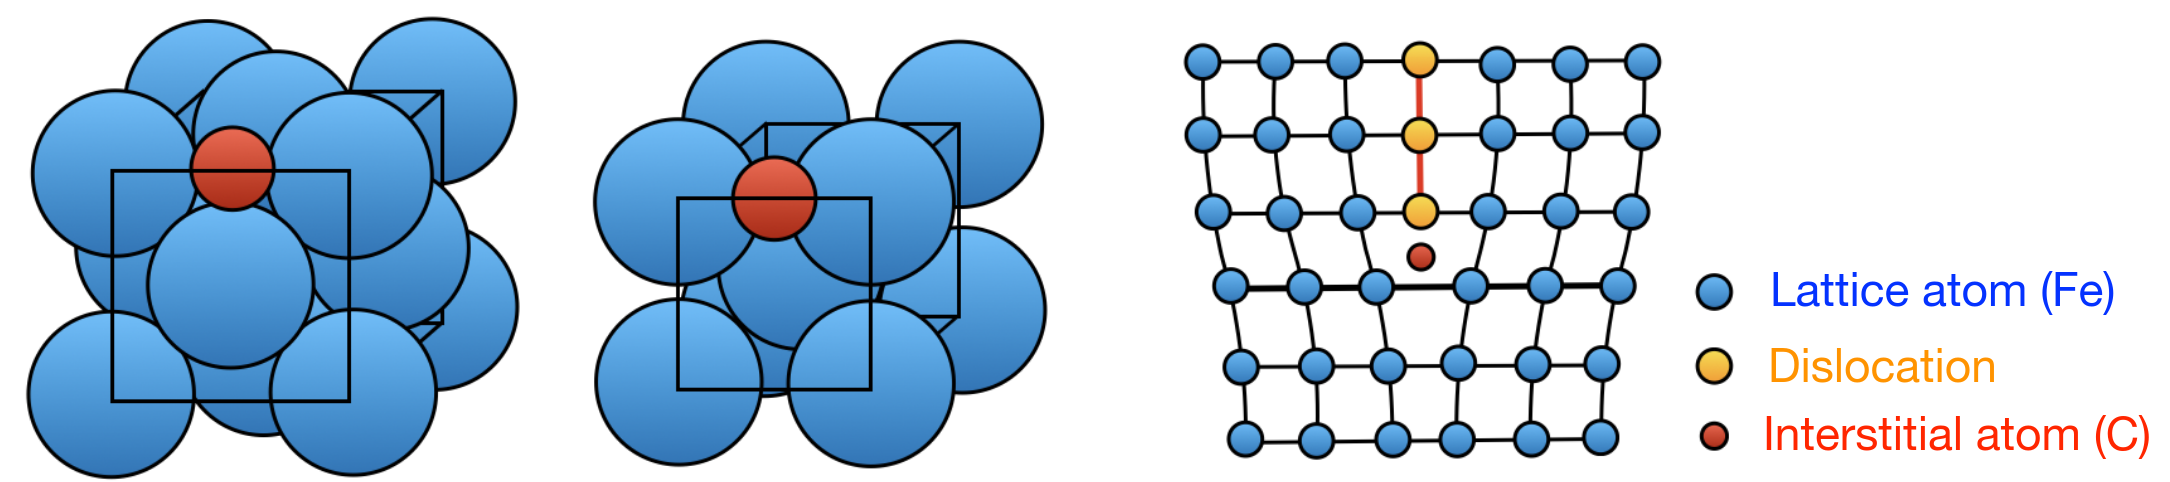
\includegraphics[width=0.8\textwidth]{media/cottrell_atmospheres.png}
  \caption*\\\vspace*{-0.25cm}{Carbon atoms occupy small octahedral sites (left), preferentially diffuse to dislocation regions (center), which forms Cottrell atmospheres that pin dislocations (right)}
\end{figure*}

\section{Strengthening mechanisms}

































\newpage
\appendix
\printacronyms[name=Glossary, heading=section]

\end{document}
